\cchapter{کارهای مرتبط}

\begin{figure}
	\centering
	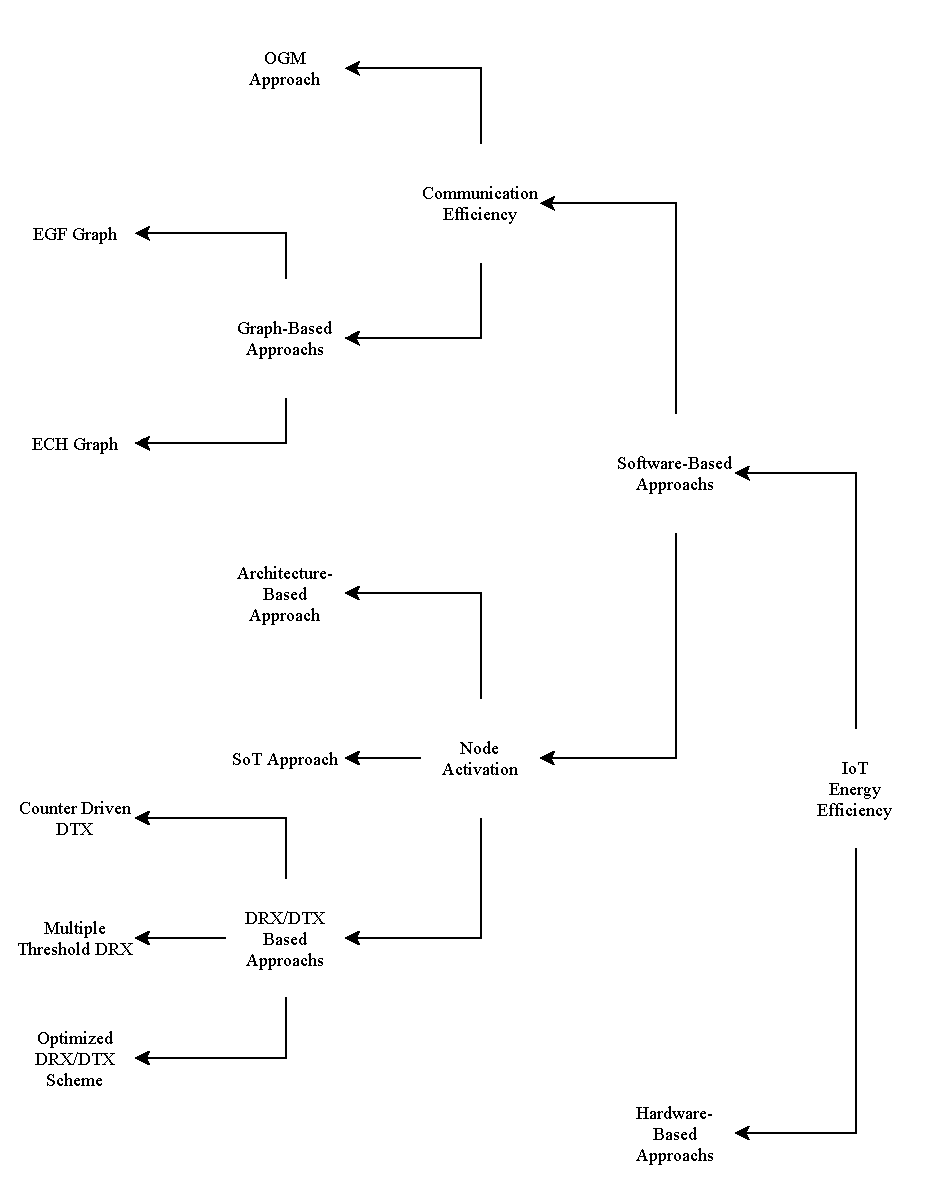
\includegraphics[width=0.9\linewidth]{figs/subject-tree}
	\caption {درخت موضوعی تحقیق}
	\label{fig:subject-tree}
\end{figure}

\par
در این بخش به بیان ایده‌های مطرح شده در مقاله‌های تحت‌بررسی می‌پردازیم. شکل \ref{fig:subject-tree} نمایان‌گر درخت موضوعی تحقیق است و همان‌طور که در تصویر مشاهده می‌نمایید؛ اساسا راهکارهای ارائه شده برای کاهش مصرف انرژی در سیستم‌های مبتنی بر اینترنت اشیا، به دو دسته‌ی کلی راهکارهای نرم‌افزاری و سخت‌افزاری تقسیم می‌گردد. در راهکارهای نرم‌افزاری، دو ایده‌ی اصلی مطرح بوده است که این ایده‌ها به ترتیب هدفشان بهینگی ارتباطات میان اجزای سیستم به منظور کاهش اتلاف انرژی در جریان انتقال داده‌ها و دیگری، غیرفعال نمودن اجزا (در این‌جا بیشتر منظور حسگرها می‌باشند.) در شرایط غیرضروری جهت کاهش مصرف انرژی توسط آن‌ها است.
\par
برای رویکرد، اول در برخی مقالات، روش‌های مبتنی بر گراف معرفی شده است که بهینگی ارتباطات سیستم را مورد هدف قرار داده‌اند. در ارتباط با رویکرد دوم نیز، معماری‌هایی ارائه شده که در آن‌ها فعال و یا غیرفعال بودن حسگرها بنابر ایده‌ی ابتکاری ارائه شده تعیین می‌گردد. علاوه بر معماری‌های ارائه شده، در برخی مقالات از مکانیزم \lr{DRX/DTX} برای فعال و غیرفعال نمودن حسگرها استفاده شده است. در ادامه به بررسی و تشریح هر یک از راهکارهای زیر خواهیم پرداخت.

\section{راهکارهای مبتنی بر مکانیزم \lr{DRX/DTX}}
پیشتر در ارتباط با مکانیزم \lr{DRX/DTX} به تفصیل صحبت کرده‌ایم. حال می‌خواهیم مقالاتی را که از این مکانیزم در بیان راهکارهایشان استفاده کرده‌اند، مورد بررسی قرار دهیم.

\subsection{\lr{Counter Driven DRX (CDD)}}
اولین راهکاری که مورد بررسی قرار می‌دهیم، راهکاری است که در مقاله \cite{} مطرح گردیده. همانطور که پیشتر نیز گفتیم، یک \lr{Trade-Off} مابین مصرف انرژی و دقت سیستم وجود دارد که می‌توان گفت این مقاله سعی در جهت ایجاد توازن در این امر را دارد. در این مقاله، هر یک از گره‌ها برای ارتباط با گره دیگر، دارای دو شمارنده هستند. در ادامه نحوه عملکرد هر یک از آن‌ها را تشریح می‌نماییم.
\par
برای بیان نحوه کارکرد این شمارنده‌ها لازم است ابتدا با نحوه عملکرد اجزای سیستم آشنایی یابیم. در یک سیستم مبتنی بر \lr{DRX/DTX}، یک گره در زمان معینی بیدار می‌شود (فعالیت خود را آغاز می‌کند)، در زمانی که فعال است به درخواست‌های رسیده از جانب دیگر گره‌ها پاسخ می‌دهد و پس از پایان زمان فعالیت مجددا به خواب می‌رود (غیرفعال می‌شود). حال اگر گره، در زمانی از خواب بیدار شود و در تمام طول مدتی که فعال است درخواستی از جانب دیگر گره‌ها دریافت ننماید، شمارنده‌ی اول خود را افزایش می‌دهد. اما اگر در یکی از زمان‌های فعالیت، گره درخواستی از دریافت نماید این شمارنده به مقدار اولیه (یا همان صفر) \lr{Reset} می‌گردد. پس از آن‌که مقدار این شمارنده از یک حدحساب\LTRfootnote{Threshold} عبور کرد؛ زمان دوره \lr{DRX} افزایش می‌یابد. همان‌طور که در فصل قبل نیز به آن اشاره شد، با افزایش زمان دوره در این مکانیزم، در واقع زمان فیرفعال بودن گره افزایش می‌یابد. در نتیجه این سیستم در واکنش به کمبودن در خواست برای یک گره (یا همان حسگر)، فعالیت آن را کاهش داده تا در مصرف انرژی صرفه‌جویی نماید. در شکل \ref{fig:cdd-extend} نمونه فعالیت این راهکار را برای افزایش زمان غیرفعال بودن یک گره مشاهده می‌کنید.

\begin{figure}
	\centering
	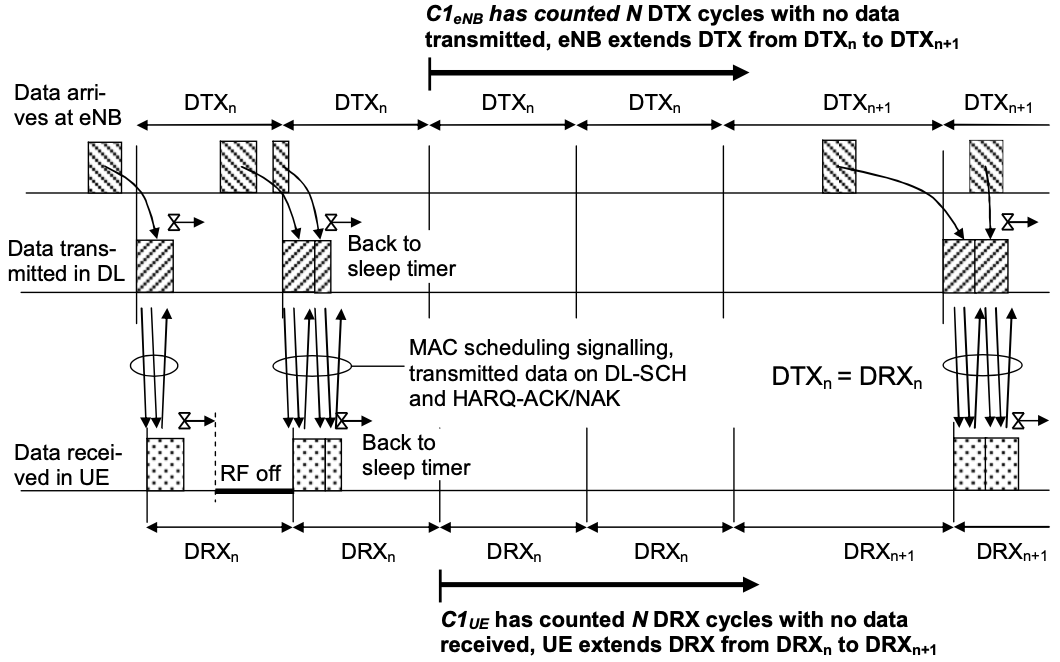
\includegraphics[width=0.7\linewidth]{figs/cdd-extend}
	\caption {افزایش دوره DRX در واکنش به کمبود درخواست برای گره}
	\label{fig:cdd-extend}
\end{figure}

\begin{figure}
	\centering
	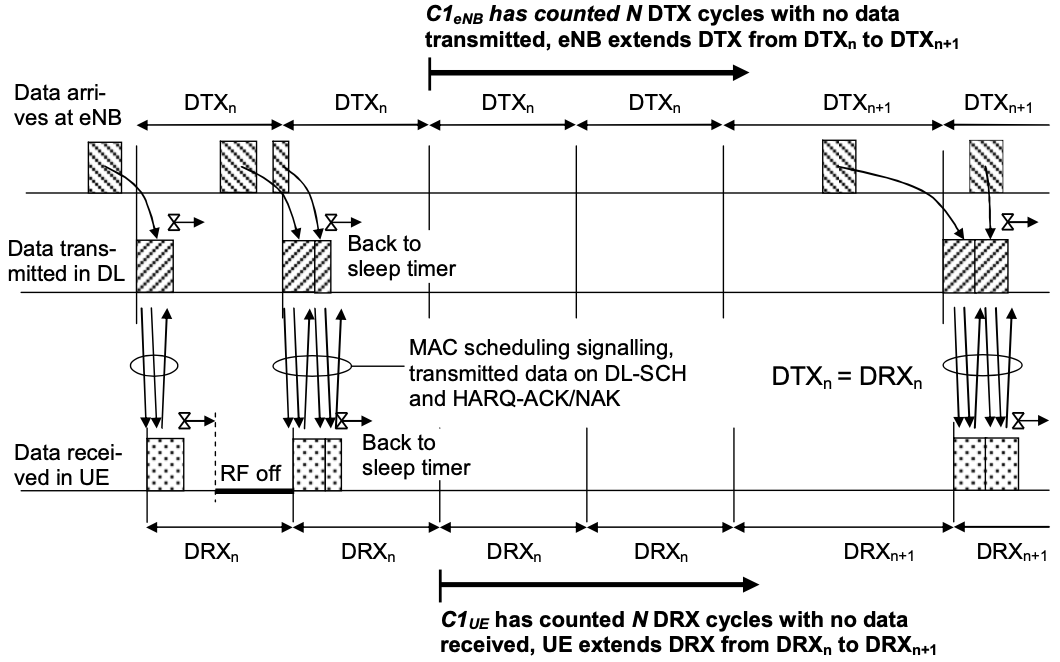
\includegraphics[width=0.7\linewidth]{figs/cdd-extend}
	\caption {کاهش دوره DRX در واکنش به ازدیاد درخواست برای گره}
	\label{fig:cdd-reduce}
\end{figure}

\par
تا این‌جا رویکرد راهکار ارائه شده در واکنش به عدم نیاز به جمع‌آوری داده از یک حسگر را دیدیم. حال به بررسی دومین شمارنده می‌پردازیم. در این شمارنده که به نوعی می‌توان گفت عکس عمل شمارنده‌ی اول را انجام می‌دهد؛ در هر دوره که گره، بیدار می‌شود؛ در صورتی که در زمان بیداری درخواستی جهت پاسخگویی به گره ارسال شده باشد، شمارنده یک واحد افزایش می‌یابد و در صورتی که درخواستی برای گره ارسال نشود، مقدار شمارنده به صفر \lr{Reset} خواهد شد. همانند شمارنده‌ی قبل؛ برای این شمارنده نیز حدحسابی درنظر گرفته شده است که اگه مقدار شمارنده از این حدحساب عبور کند، دوره تناوب گره کاهش می‌یابد. همان‌طور که گفته شد، این عمل برعکس عمل شمارنده‌ی بالاست. یعنی به کمک این شمارنده، سیستم متوجه می‌شود که گره در هر دوره‌ی بیداری درخواستی برای پاسخگویی داشته و در نتیجه، سیستم درمی‌یابد که نیازمندی سیستم به این گره بیش از مقدار فعلی است. پس برای افزایش دقت سیستم لازم است تا گره با تناوب کوتاه‌تری به فعالیت بپردازد  که البته همان‌طور که پیشتر هم اشاره شده این امر موجب افزایش انرژی مصرفی گره و در ازای آن، کاهش طول عمر سیستم می‌شود. در شکل \ref{fig:cdd-reduce} نمونه فرآیند کاهش طول دوره برای یک گره را مشاهده می‌نمایید.

\subsubsection{نیرومندی راهکار ارائه شده}
منظور از نیرومندی\LTRfootnote{Robustness} راهکار ارائه شده، اثبات عملکرد آن در ازای بروز هرگونه خطا می‌باشد. به همین منظور، در مقاله مذکور مجموعا چهار نوع خطا در حین کارکرد سیستم ارزیابی شده است. که به شرح ذیل می‌باشند.
\begin{enumerate}
	\item{
	گره درخواست‌کننده، درخواست را زمانبندی می‌کند. اما در ارسال موفق نمی‌شود. گره پاسخگو، سیگنال منفی (\lr{NAK}) در پاسخ می‌فرستد.
	}
	\item{
	گره درخواست‌کننده، درخواست را زمان‌بندی و ارسال می‌کند. گره پاسخگو، سیگنال را با خطا می‌فرستد.
	}
	\item{
گره درخواست‌کننده، برای ارسال درخواست دچار خطا می‌شود و گره پاسخگو نیز در ارسال سیگنال پاسخ دچار خطا می‌گردد.
	}
	\item{
گره درخواست‌کننده، در زمان‌بندی و ارسال درخواست دچار خطا می‌شود و طبیعتا به دلیل خطای زمان‌بندی، امکان ارسال سیگنال از جانب گره پاسخگو وجود ندارد.
	}
\end{enumerate}

\par
خطاهای ذکر شده در بالا را می‌توانید در شکل \ref{fig:cdd-errors} مشاهده نمایید. همانگونه که در تصویر نیز مشهود است؛ در صورت بروز هر یک از خطا دو سیستم از نقطه $A$ به بعد مجددا با هم همگام شده و عملکرد طبیعی سیستم مشاهده می‌گردد.

\begin{figure}
	\centering
	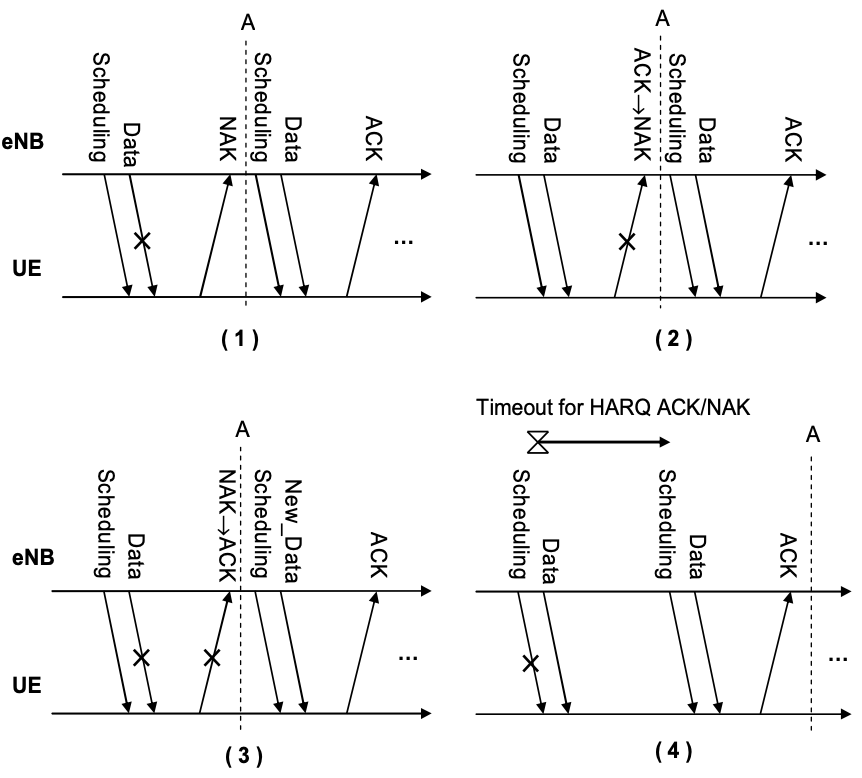
\includegraphics[width=0.8\linewidth]{figs/cdd-errors}
	\caption {خطاهای ممکن در حین برقرار ارتباط میان دو گره}
	\label{fig:cdd-errors}
\end{figure}

\subsection{\lr{Multiple Threshold DRX (MTD)}}
راهکار ارائه شده در این مقاله\cite{}، این است که برخلاف راهکار ارائه شده در مقاله‌ی قبل، تغییری در طول دوره‌ی گره ایجاد نمی‌شود؛ بلکه بر اساس شیوه‌ای به تغییر مقدار زمان \lr{Inactivity Timer} گره می‌پردازد. در مورد این پارامتر نیز در فصل پیش به تفصیل صحبت کردیم اما برای یادآوری، این پارامتر بیانگر مدت زمانی بود که گره، پس از دریافت درخواست از جانب سایر گره‌ها روشن می‌ماند تا درخواست رسیده را پاسخ دهد و در این مدت به سایر درخواست‌های رسیده پاسخگو نبود.
\par
در راهکار ارائه شده در مقاله مورد بررسی، ۱۰ حالت برای کیفیت عملکرد گره‌ها در نظر گرفته شده است که از حالت ۱ الی ۱۰ زمان \lr{Inactivity Timer} آن‌ها افزوده شده و در نتیجه کیفیت عملکرد آن‌ها کاهش می‌یابد. دلیل کاهش کیفیت عملکرد از دیدگاه این مقاله، این است که با افزایش زمان \lr{Inactivity Timer}، امکان دریافت درخواست‌های جدید از گره سلب می‌شود و دقت کاهش می‌یابد. پس در نتیجه، حالت ۱ باکیفیت‌ترین و حالت ۱۰ کم‌کیفیت‌ترین حالت است. این حالات را می‌توانید در جدول \ref{tbl:mtd} مشاهده نمایید. در ابتدا، تمامی گره‌ها در حالت ۱ قرار دارند. پس از آن‌، به طور متاوب، شاخص کیفیت (\lr{CQI}\RTLfootnote{مخفف \lr{Channel Quality Indicator}}) هر یک از گره‌ها محاسبه می‌شود.
پس از محاسبه‌ی \lr{CQI} هریک از حالات مذکور دارای یک حدحساب \lr{CQI} است که این حدحساب‌ها در شکل \ref{fig:mtd} قابل‌مشاهده است. اگر در مدت‌زمان $T\_trig$ که در جدول \ref{tbl:mtd} آمده است، مقدار \lr{CQI} پایین‌تر از حدحساب باشد، گره از حالت فعلی به یک حالت بالاتر می‌رود و در نتیجه تایمر طولانی‌تر شده که منجر به کاهش کیفیت عملکرد و البته، افزایش طول عمر گره می‌گردد.
\par
برعکس همین عمل نیز در سیستم اتفاق می‌افتد. یعنی اگر برای یک گره، در ازای مدت‌زمان بیشتری از $T\_trig$ میزان \lr{CQI} بالاتر از حدحساب حالت کمتر (باکیفیت‌تر) باشد، حالت کیفیت گره به حالت باکیفیت‌تر تقلیل می‌یابد که موجب افزایش دقت عملکرد حسگر می‌گردد.

\begin{figure}
	\centering
	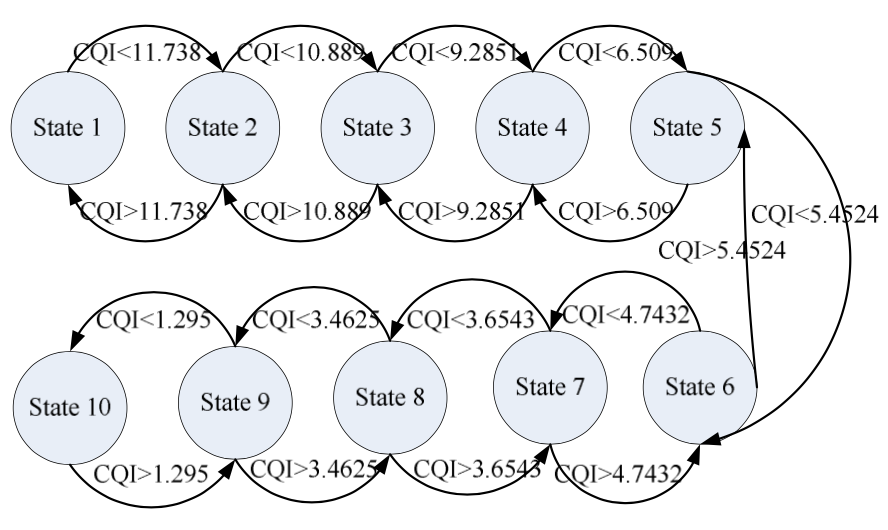
\includegraphics[width=0.7\linewidth]{figs/mtd}
	\caption {حالت‌های کیفیت در MTD و حدحساب هر یک}
	\label{fig:mtd}
\end{figure}

\begin{table}
	\begin{center}
		\caption{مقادیر تایمر مربوط به هر یک از حالات}
		\label{tbl:mtd}
		\begin{tabular}{|p{0.3\linewidth}|p{0.4\linewidth}|}
			\hline
			\textbf{پارامتر} & \textbf{DRX Inactivity Timer (TTI)}\\
			\hline
			حالت ۱ & $4$\\
			\hline
				حالت ۲ & $5$\\
			\hline
				حالت ۳ & $10$\\
			\hline
				حالت ۴ & $20$\\
			\hline
				حالت ۵ & $30$\\
			\hline
				حالت ۶ & $40$\\
			\hline
				حالت ۷ & $50$\\
			\hline
				حالت ۸ & $60$\\
			\hline
				حالت ۹ & $80$\\
			\hline
				حالت ۱۰ & $100$\\
			\hline
			\lr{\textbf{T\_trig}} & $6$\\
			\hline
		\end{tabular}
	\end{center}
\end{table}

\subsection{Optimized DRX/DTX}
راهکار ارائه شده در مقاله \cite{}، از بسیاری جهات از راهکار‌های ارائه شده در دو مقاله‌ی اول در زمینه استفاده از \lr{DRX/DTX} برای کاهش مصرف انرژی، بهینه‌تر است. در این مقاله، راهکار ارائه شده به این صورت است که ابتدا، بر اساس مدت زمان قابل‌قبول (بودجه زمانی) جریان‌\LTRfootnote{Flow}‌های داده مرتبط با یک گره، دوره‌ی کوتاه آن و سپس دوره‌ی بلند‌مدت آن را تعیین می‌نماید. سپس بر اساس پارمتر‌های تعیین شده، مقادیر \lr{On Duration} و \lr{Inactivity Timer} به‌ دست ‌می‌آید.

\subsubsection{تعیین زمان دوره}
در اولین گام از این راهکار، همان‌طور که گفته شد، به تعیین مقدار زمان دوره‌ی کوتاه (یا همان \lr{Short Cycle}) می‌پردازیم. بر این اساس، ابتدا باید اضطراری‌ترین جریان داده را مشخص نماییم. اضطراری‌ترین جریان داده، جریانی‌است که بودجه زمانی کمتری داشته و به عبارت دیگر انتظار می‌رود تا در زمان کمتری از جانب گره پاسخ یابد. این پارمتر را برای گره‌ی $i$ با نماد $D^{min}_i$ نمایش می‌دهیم. مدت زمان دوره‌ی کوتاه به وسیله‌ی فرمول \ref{eq:drx-short-cycle} محاسبه می‌شود.

\begin{equation}
T^S_i = \left\lfloor \frac{D^{min}_i}{T^S_{i-1}} \right\rfloor . T^S_{i-1}
\label{eq:drx-short-cycle}
\end{equation}

در فرمول بالا همان‌طور که مشاهده می‌شود، زمان به دست آمده از $D^{min}_i$ کوچکتر و یا مساوی با آن است. پس حتی امکان پاسخ‌دهی جریان داده‌ای با کمترین زمان قابل‌قبول را نیز ارضا می‌کند و هیچ جریان داده‌ای به واسطه طولانی بودن زمان دوره از دست نمی‌رود (\lr{Miss} نمی‌شود). حال، برای به دست آوردن مدت زمان دوره‌ی طولانی مدت، ابتدا در بین سرویس‌های مرتبط با گره، کوتاه‌ترین زمان پاسخگویی قابل‌قبول را یافته و بر اساس فرمول \ref{eq:drx-long-cycle}، محاسبه‌ی زمان دوره را انجام می‌دهیم. کوتاه‌ترین زمان پاسخگویی قابل‌قبول را برای گره $i$ با نماد $S^{min}_i$ نمایش می‌دهیم.

\begin{equation}
T^L_i = \left\lfloor \frac{S^{min}_i}{T^S_i} \right\rfloor . T^S_i
\label{eq:drx-long-cycle}
\end{equation}

همانطور که در فرمول فوق مشاهده می‌شود، مدت‌زمان دوره‌ی طولانی یک گره، در واقع ضریبی از مدت‌زمان دوره‌ی کوتاه آن می‌باشد. علاوه بر این، گزاره‌ی بالایی در مورد این فرمول نیز کاربرد دارد. یعنی به دلیل آن که $T^L_i$ کوچکتر و یا مساوی $S^{min}_i$ است، در نتیجه حتی کوتاه‌ترین زمان در میان زمان‌های قابل‌قبول برای پاسخ‌دهی به سرویس‌های مرتبط با گره را نیز ارضا خواهد کرد و به عبارت دیگر، سرویسی به دلیل طولانی بودن زمان دوره از دست نخواهد رفت.

\subsubsection{تعیین مدت‌زمان \lr{On Duration} و \lr{Inactivity Timer}}
برای محاسبه‌ی مدت‌زمان \lr{On Duration} راهکار ارائه شده به این صورت است که مجموع بیشینه‌ی حجم بسته‌ی جریان‌هایی را در نظر می‌گیریم که بودجه‌ی زمانی‌شان، برابر با مدت‌زمان دوره‌ی کوتاه که در مرحله‌ی قبل محاسبه کردیم باشد. سپس این مقدار را بر حداقل میزان کانال\LTRfootnote{Channel} گره‌ی مدنظر تقسیم می‌نماییم. لازم به ذکر است که مقدار از ضرب $\Omega$ که بیانگر تعداد بلوک‌های منبع\LTRfootnote{Resource Block (RB)} است در $C^{min}_i$ که بیانگر حداقل نرخ کانال\LTRfootnote{Channel Rate} بوده و واحد آن نیز (\lr{bits/RB}) می‌باشد، محاسبه می‌شود. علاوه بر این، همان‌طور که در فرمول \ref{eq:drx-on-duration} مشاهده می‌شود؛ یک مقدار حداقلی (در اینجا ۱) نیز برای محاسبه زمان \lr{On Duration} در نظر گرفته می‌شود.

\begin{equation}
O_i = \max \left\{ \left\lceil \frac{\Sigma_{D_j = T^S_i, \forall flow_j \in U E_i} Q^{max}_j}{C^{min}_i \times \Omega} \right\rceil , 1 \right\}
\label{eq:drx-on-duration}
\end{equation}

\par
دلیل چنین رویکردی این است که مطمئن باشیم حتی با کمترین منابع، در مدت زمان \lr{On Duration} قادر به دریافت تمام بسته‌های جریان داده هستیم.

\par
اما برای محاسبه \lr{Inactivity Timer}، ابتدا لازم است تا \lr{expected packet loss rate} را که آن را با نماد $E_{i, j}$ نمایش می‌دهیم، برای هر گره $i$ و هر جریان داده‌ای $j$ محاسبه کنیم. با فرض این که تعداد بسته‌های مربوط به یک جریان داده، $M_j$ عدد باشد و هر کدام از این بسته‌ها دارای تاخیری در بازه‌ی $1..D_j$ باشد، (اگر بیش از $D_j$ یا همان بودجه‌ی زمانی تاخیر داشته باشیم اصولا بسته از دست رفته است) مقدار $E_{i, j}$ از فرمول \ref{eq:drx-eij} محاسبه می‌شود.

\begin{equation}
E_{i, j} = \sum^{M_j}_{t_m = 1..D_j, m} Prob(t_m) \times Loss(m)
\label{eq:drx-eij}
\end{equation}

\begin{equation}
Loss(m) = \frac{M_j - \left(\Sigma_{m = 1..M_j}(\phi_m + \eta_m)\right)}{M_j}
\label{eq:drx-loss}
\end{equation}

\begin{equation}
\phi_m = 
\begin{cases}
	1, &$if$ \; X_m \leq D_j\\
	0, &$otherwise$
\end{cases}
\label{eq:drx-phi}
\end{equation}

\begin{equation}
\eta_m = 
\begin{cases}
	1, &$if$ \; X_m > D_j \; $and$ \; Y_m \leq \hat{\Gamma}^I_j \\
	0, &$otherwise$
\end{cases}
\label{eq:drx-eta}
\end{equation}

\par
تابع $Prob$ به صورت شهودی از سیستم به دست می‌آید و فرمول $Loss$ در \ref{eq:drx-loss} آمده است. برای محاسبه این تابع برای بسته‌ی $m$، به دو پارامتر نیاز است که این پارامترها به ترتیب $\phi_m$ و $\eta_m$ می‌باشند. پارامتر اول که در فرمول \ref{eq:drx-phi} آمده است، بیانگر این است که آیا بسته در زمان \lr{On Duration} گره قابل دریافت است یا خیر و پارامتر دوم که در فرمول \ref{eq:drx-eta} به آن اشاره گردیده است، بیانگر این امر است که آیا بسته در زمان  \lr{Inactivity Timer} قابل دریافت است یا خیر. مجموع این دو پارامتر اگر برابر با یک باشد به این معنی است که بسته از جانب گره قابل دریافت بوده است.  همان‌طور که مشاهده می‌شود، در فرمول \ref{eq:drx-loss} از مجموع این دو پارامتر استفاده گردیده است تا احتمال دریافت بسته سنجیده شود.

\par
پس از محاسبه‌ی تمامی $E_{i, j}$ها، برای هر جریان داده‌ی $j$ مقدار کمینه $E_{i, j}$ به عنوان مقدار کاندید \lr{Inactivity Timer} انتخاب می‌شود. لازم به ذکر است که دلیل انتخاب مقدار کمینه، این است که مقدار $P^{loss}_{i, j}$ (این پارامتر، بیانگر میزان قابل‌قبول \lr{Loss} شدن بسته‌های جریان $j$ در گره $i$ می‌باشد) ثابت بوده و در نتیجه تاثیری در \lr{Loss} شدن بسته‌ها ندارد؛ پس بدیهی است که کمترین مقدار \lr{Inactivity Timer}، به دلیل کمتر بیدار بودن گره، باعث کاهش مصرف انرژی می‌شود. سپس از بین تمامی کاندیدهای انتخاب شده، بیشترین مقدار به عنوان \lr{Inactivity Timer} گره موردنظر انتخاب می‌گردد. دلیل انتخاب مقدار بیشینه در این مرحله، این است که مقدار انتخاب شده به ازای تمامی جریان‌های داده قابل‌قبول باشد و به عبارت دیگر، مقدار نهایی \lr{Inactivity Timer} ،$P^{loss}_{i, j}$ مرتبط با همه‌ی جریان‌های داده گره را ارضا کند. 

\subsubsection{زمان‌بندی بسته‌ها}
علاوه بر استفاده از مکانیزم \lr{DRX/DTX} در مقاله‌ی مورد بررسی، یکی دیگر از ایده‌های مطرح شده در این مقاله، استفاده از یک مکانیزم ابداعی جهت زمان‌بندی بسته‌ها می‌باشد. در این مکانیزم بسته‌های مرتبط با هر گره، در یک صف در گره کنترل‌کننده نگه‌داری می‌شود. سپس گره‌کننده، بلوک منبعی را به هر یک از گره‌هایی که بسته‌ای جهت پردازش داشته باشند و زمان \lr{Inactivity Timer} آن‌ها رو به اتمام باشد؛ تخصیص می‌دهد. سپس بلوک‌های باقی‌مانده مابین گره‌های دیگر که اولویت پایین‌تری دارند تقسیم می‌شود. این عمل منجر به افزایش کیفیت سیستم شده و احتمال \lr{Loss} شدن بسته‌های داده‌ای جریان‌های گره را کاهش می‌دهد.

\section{راهکارهای مبتنی بر گراف}
در مقالاتی که در ادامه به بررسی آن‌ها خواهیم پرداخت، ایده‌ی اصلی مطرح شده، استفاده از گراف‌های درختی برای کاهش فواصل میان گره‌های شبکه می‌باشد. این کاهش فاصله منجر به کاهش مصرف انرژی به هنگام ارسال و دریافت اطلاعات میان گره‌ها می‌شود. در ادامه به بررسی راهکار مقاله‌ی اول از این دسته خواهیم پرداخت.

\subsection{درخت EGF}
در مقاله \cite{} راهکاری که ارائه شده، این است که محیط سیستم مبتنی بر اینترنت اشیا به لحاظ جغرافیایی به نواحی‌ای از محیط‌های محلی خوشه‌بندی شود که در هر یک از آن‌ها یک گره به عنوان گره سرگروه فعالیت می‌کند. وظیفه‌ی گره سرگروه این است که ارتباط لازم میان گره هدف و \lr{Base Station} را برقرار نماید. به این وسیله مصرف انرژی شبکه مبتنی بر اینترنت اشیا کاهش چشمگیری می‌یابد. زیرا در هنگام برقراری ارتباط، نیازی به روشن بودن مدار ارتباطی همه گره‌ها نیست و نکته‌ی اصلی همین است که بخش زیادی از انرژی مصرف شده توسط گره‌ها مربوط به مدار ارتباطی آن‌ها می باشد.

\subsubsection{مدل انرژی}
در مقاله‌ی مذکور برای مدل‌سازی ریاضی انرژی از توابع زیر استفاده شده است. لازم به ذکر است که فرمول \ref{eq:egf-etx} بیانگر میزان انرژی لازم برای ارسال $k$ بیت پیام به فاصله‌ی $d$، فرمول \ref{eq:egf-erx} بیانگر میزان انرژی مصرفی جهت دریافت $k$ بیت پیام و فرمول \ref{eq:egf-energy} بیانگر میزان انرژی لازم برای انتقال (ارسال و دریافت) $k$ بیت پیام به فاصله $d$ می‌باشد.

\begin{equation}
E_{tx} = a \times k + b \times k \times d^n_{ij}
\label{eq:egf-etx}
\end{equation}

\begin{equation}
E_{rx} = c \times k
\label{eq:egf-erx}
\end{equation}

\begin{equation}
C_{ij}(K) = 
\begin{cases}
	a \times k + b \times k \times d^n_{ij} & $if$ \; j \; $is$ \; BS\\
	E_{tx} + E_{rx} & $otherwise$
\end{cases}
\label{eq:egf-energy}
\end{equation}

\par
همان‌گونه که در فرمول‌های بالا ملاحظه ‌می‌شود؛ $a$، $b$ و $c$ ثابت هستند  و $d_{ij}$ بیانگر فاصله‌ي میان دو گره $i$ و $j$ است. علاوه بر این، این نکته از فرمول‌های بالا برداشت می‌شود که دریافت پیام توسط $BS$ یا همان \lr{Base Station} محدودیتی ندارد و به همین دلیل در مدل ریاضی مقاله‌ی تحت بررسی از این مقدار چشم‌پوشی شده است.

\begin{figure}
	\centering
	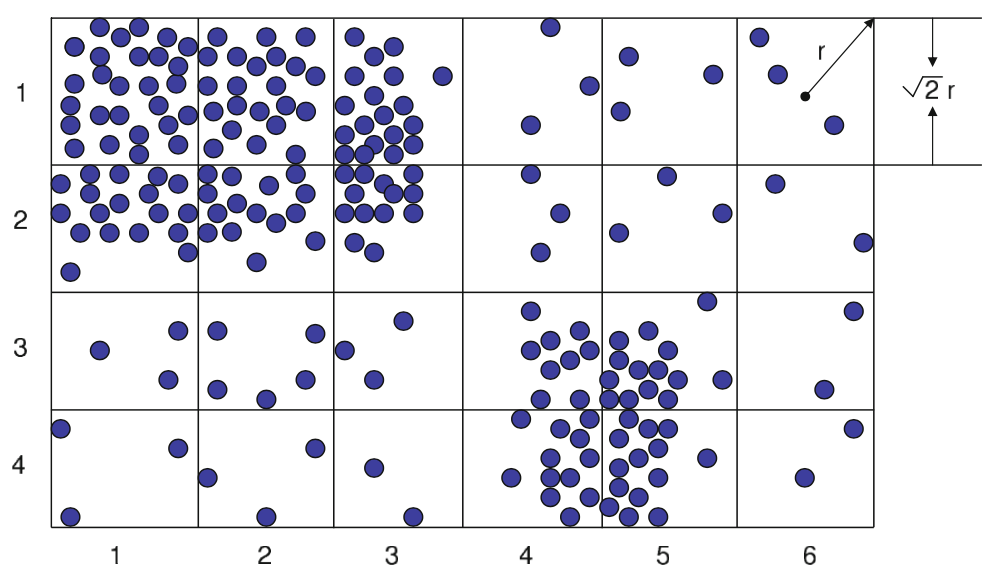
\includegraphics[width=0.7\linewidth]{figs/egf-env}
	\caption {محیط مورد بررسی در مقاله‌ی \cite{}}
	\label{fig:egf-env}
\end{figure}

\subsubsection{ساخت درخت EFG}
فرض کنید محیطی که قرار است درخت را در آن تشکیل دهیم، محیط نمایش داده شده در شکل \ref{fig:egf-env} است. برای ساخت درخت، همانطور که در الگوریتم شکل \ref{fig:egf-al1} دیده می‌شود، ابتدا محیط را به سلول\LTRfootnote{Cell}های مربعی با طول ضلع $\sqrt{2}r$ (که $r$ بیانگر شعاع ارتباطی حسگرها است و در این مقاله برای تمامی حسگرها یکسان است) تقسیم‌بندی می‌نماییم.
\par
پس از آن که تقسیم‌بندی سلول‌ها انجام گردید؛ در الگوریتم ارائه شده، نوبت به مرحله‌ی محاسبه‌ی وزن می‌رسد. در این مرحله، به ازای هر گره، وزن میان این گره و گره‌های مجاور آن (یعنی گره‌های بالا، پایین، چپ و راست گره مورد نظر) به کمک الگوریتم دوم که در شکل \ref{fig:egf-al2} مشهود است؛‌ محاسبه می‌شود. در ادامه به توضیح این الگوریتم خواهیم پرداخت.
\par
اما بعد از آن که محاسبه‌ی وزن میان سلول‌های محیط صورت گرفت؛ ابتدا تمامی سلول‌ها را به عنوان یک زیرمحیط\LTRfootnote{Sub-Region} در نظر می‌گیریم و وزن میان هر جفت از این زیرمحیط‌ها را به صورت نزولی مرتب می‌نماییم. در این مرحله، هر بار؛ دو زیرمحیط که بین‌شان بالاترین وزن موجود است با یکدیگر ادغام کرده و یک زیرمحیط جدید ایجاد می‌کنیم که در واقع والد دو زیرمحیط قبلی است. بدین صورت گره‌های دو زیرمحیط قبلی به عنوان گره‌های فرزند\LTRfootnote{Child Nodes} زیرمحیط جدید معرفی می‌شوند.
\par
پس از آنکه زیرمحیط جدید تعریف شد، در واقع همان مرحله‌ی قبلی - که محاسبه وزن بود - باید برای آن صورت گیرد. اما با این تفاوت که این بار، وزن باید برای یک زیرمحیط محاسبه شود و نه یک سلول که روش محاسبه‌ی وزن برای زیرمحیط در الگوریتم شکل \ref{fig:egf-al3} آمده است. در مورد این الگوریتم نیز جلوتر به تفصیل صحبت می‌نماییم. سپس، با محاسبه‌ی وزن زیرمحیط‌های مجاور زیرمحیط مدنظر (زیرمحیط‌های بالا، پایین، چپ و راست آن) کار الگوریتم در گام اول به پایان می‌رسد و عملیات ذکر شده در دو پاراگراف اخیر (خط‌های ۱۰ الی ۱۷ شبه کد الگوریتم شکل \ref{fig:egf-al1}) تکرار می‌گردد. این عملیات تا آن‌جایی ادامه پیدا ‌می‌کند که دیگر فقط یک زیرمحیط در تمام محیط تحت پوشش سیستم باقی بماند.
به این صورت گراف محیط شکل \ref{fig:egf-env} ساخته شده و در شکل \ref{fig:egf-graph} قابل مشاهده است. لازم به ذکر است که در گراف درختی ساخته شده، سلول‌ها در موقعیت برگ‌های درخت قرار می‌گیرند.

\begin{figure}
	\centering
	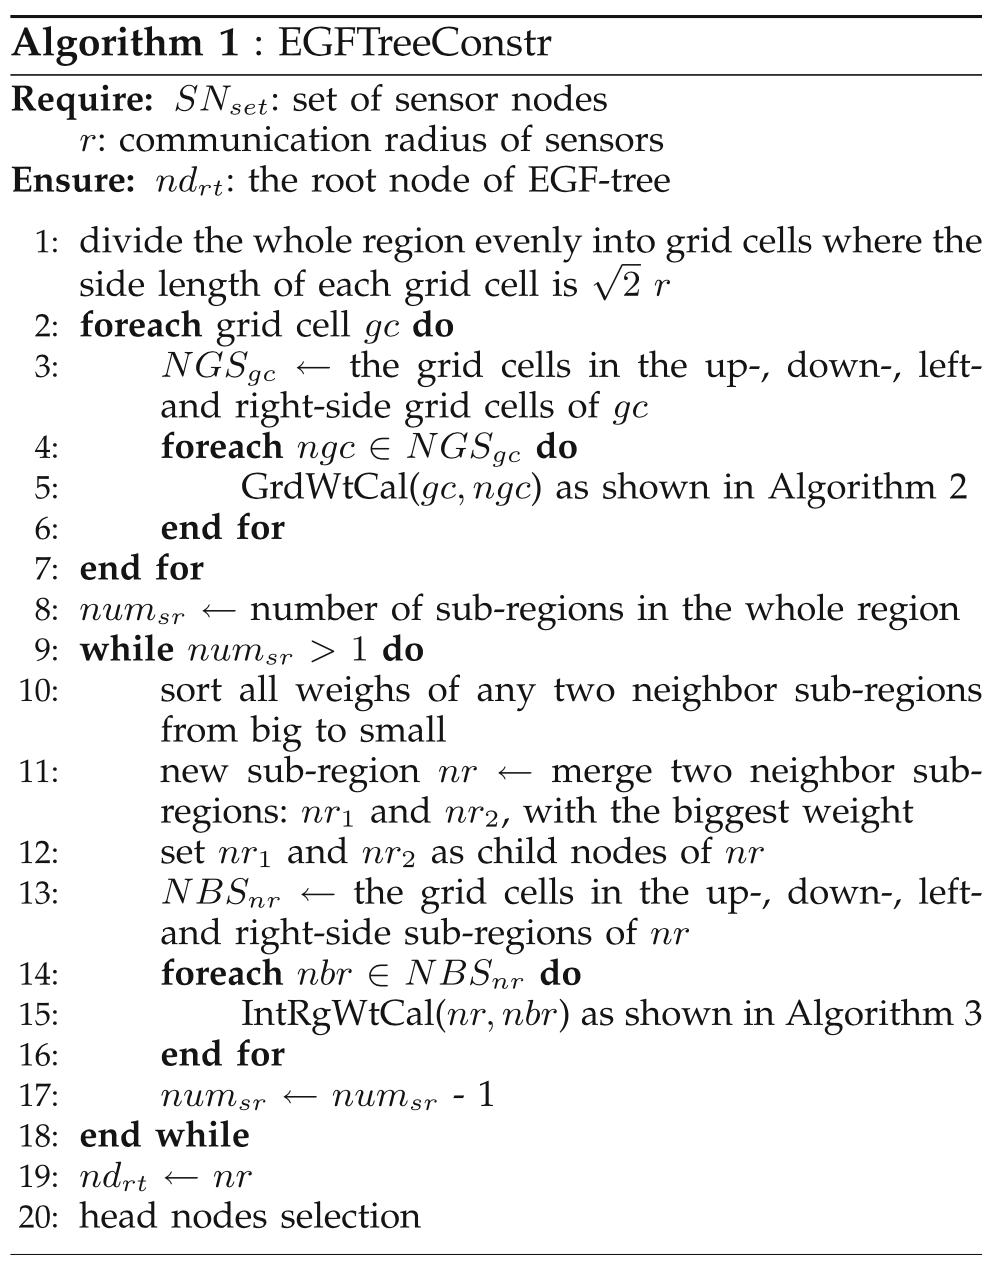
\includegraphics[width=0.7\linewidth]{figs/egf-al1}
	\caption {شبه کد الگوریتم ساخت درخت EGF}
	\label{fig:egf-al1}
\end{figure}

\begin{figure}
	\centering
	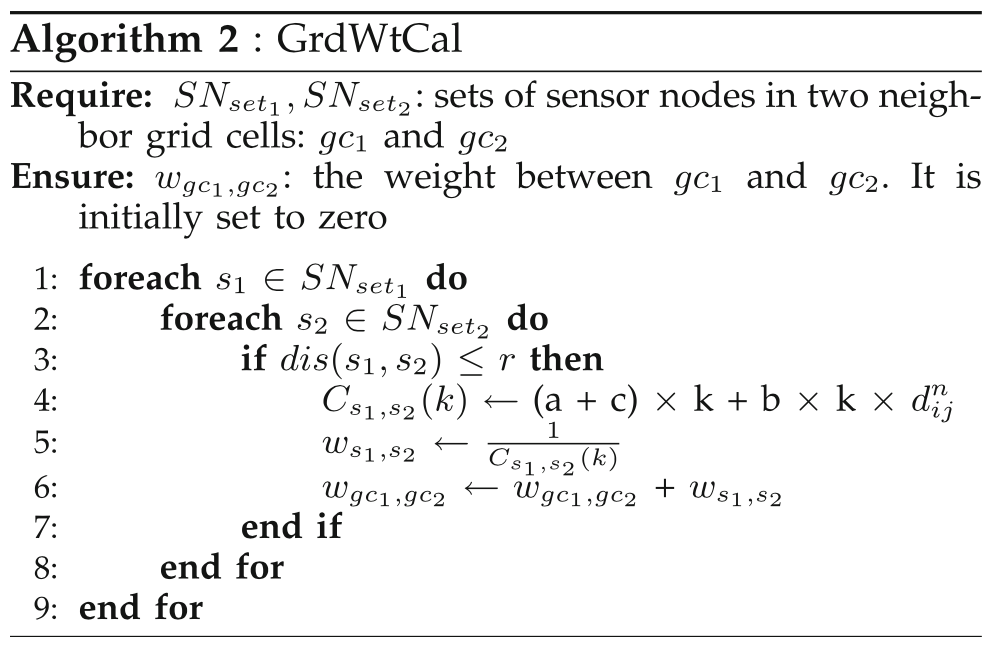
\includegraphics[width=0.7\linewidth]{figs/egf-al2}
	\caption {شبه کد الگوریتم محاسبه‌ی وزن میان سلول‌ها}
	\label{fig:egf-al2}
\end{figure}

\begin{figure}
	\centering
	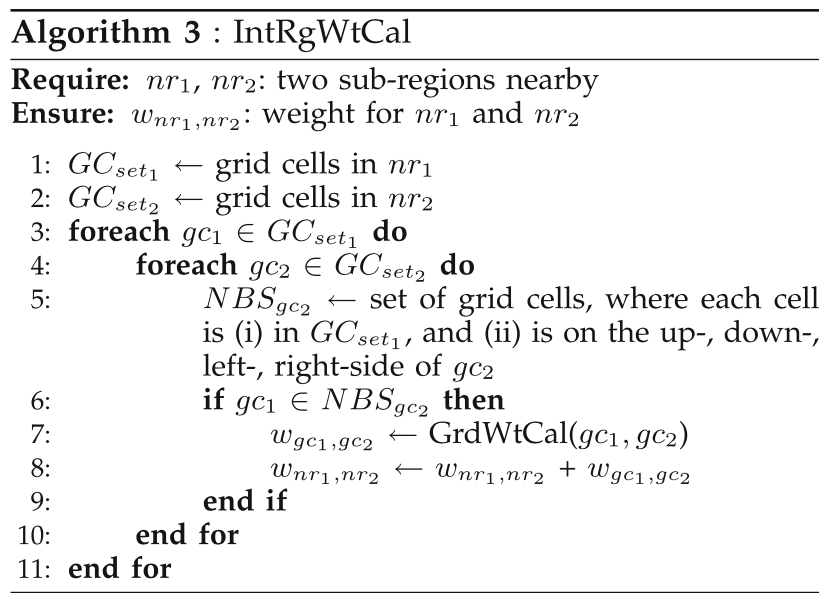
\includegraphics[width=0.7\linewidth]{figs/egf-al3}
	\caption {شبه کد الگوریتم محاسبه‌ی وزن میان زیرمحیط‌ها}
	\label{fig:egf-al3}
\end{figure}

\begin{figure}
	\centering
	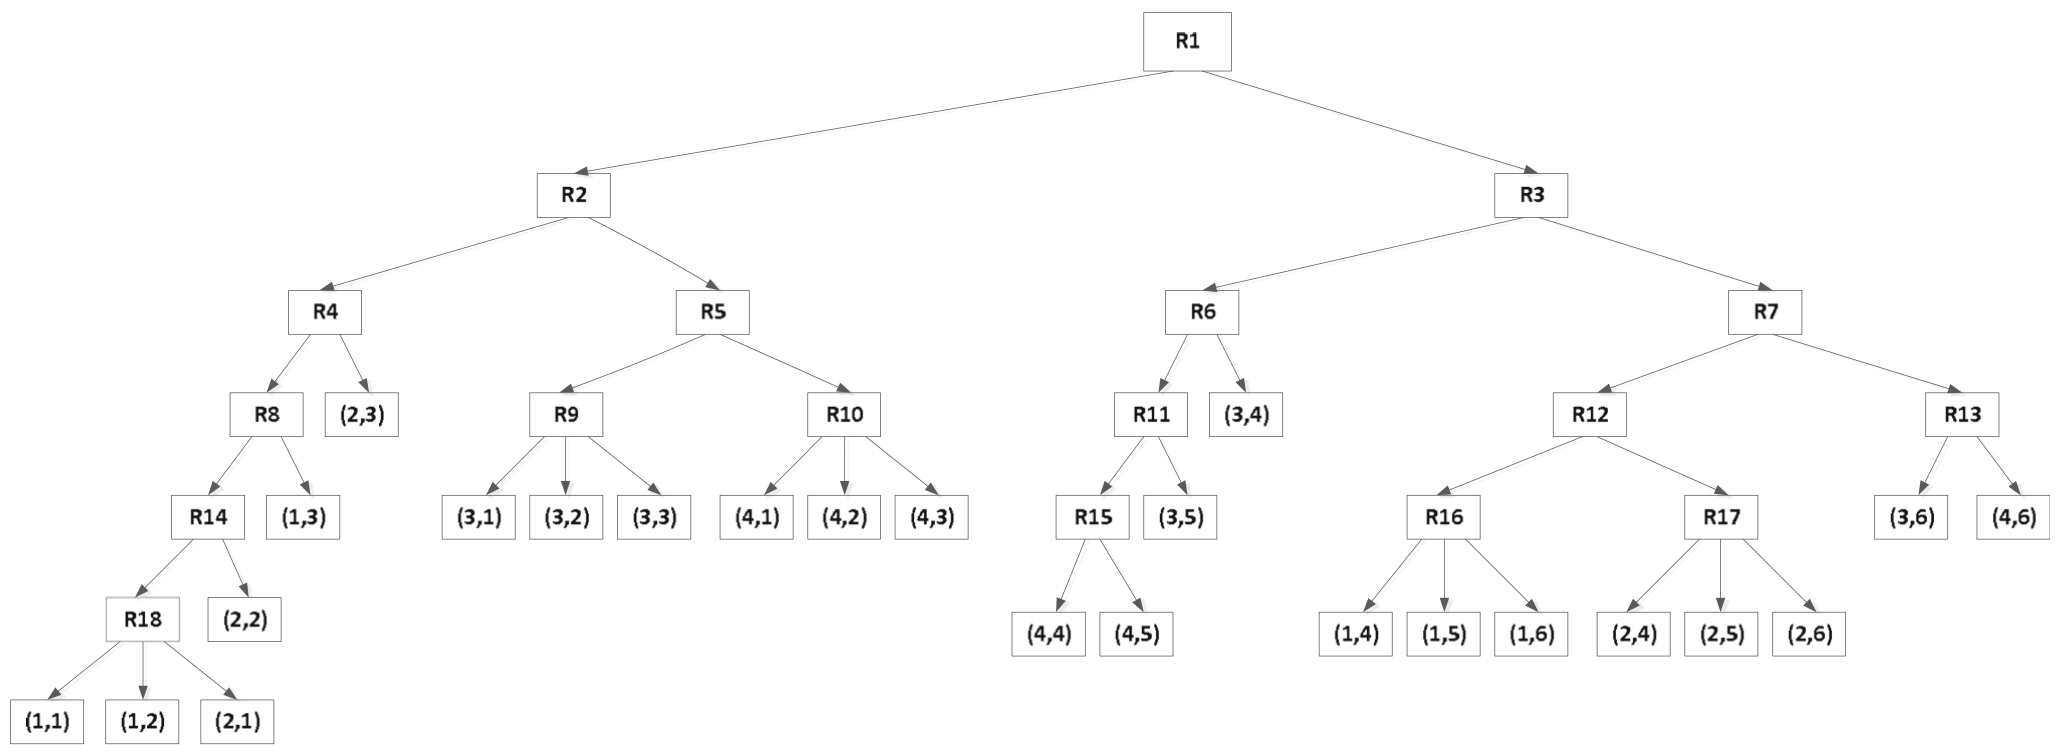
\includegraphics[width=0.7\paperheight,angle=90,origin=c]{figs/egf-graph}
	\caption {گراف حاصل شده برای محیط شکل \ref{fig:egf-env}}
	\label{fig:egf-graph}
\end{figure}

\par
در الگوریتم شکل \ref{fig:egf-al2} برای محاسبه‌ی وزن میان دو سلول مجاور، به ازای هر جفت گره‌ای از سلول اول و سلول دوم (یعنی گره اول در جفت گره موردنظر، متعلق به سلول اول و گره دوم متعلق به سلول دوم باشد) عملیات زیر را انجام می‌دهیم. ابتدا، بررسی انجام می‌شود که فاصله‌ی دو گره از هم بیشتر از شعاع ارتباطی (یا همان $r$) نباشد. سپس در صورتی که فاصله‌ی بین دو گره، کمتر و یا مساوی شعاع ارتباطی‌شان بود؛ وزن میان آن دو گره از معکوس $C_{ij}(k)$  که محاسبه‌ی آن در فرمول \ref{eq:egf-energy} شرح داده شد به دست ‌می‌آید. سپس از مجموع وزن‌های به دست آمده در میان گره‌ها، وزن کلی میان دو سلول حاصل می‌گردد. در فرمول \ref{eq:egf-weight} می‌توانید نمونه محاسبه وزن میان دو سلول قابل مشاهده در شکل \ref{fig:egf-weight} را بررسی نمایید.

\begin{equation}
w_{(3,1),(3,2)} = \frac{1}{C_{S_2,S_4}(k)} + \frac{1}{C_{S_2,S_5}(k)} + \frac{1}{C_{S_3,S_4}(k)}
\label{eq:egf-weight}
\end{equation}

\begin{figure}
	\centering
	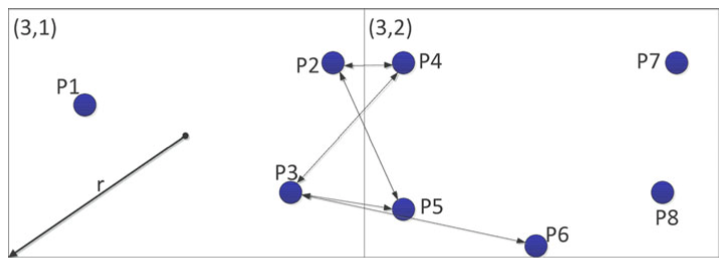
\includegraphics[width=0.7\linewidth]{figs/egf-weight}
	\caption {محاسبه‌ی وزن میان دو سلول مجاور}
	\label{fig:egf-weight}
\end{figure}

\par
از فرمول بالا می‌توان دریافت که فاصله‌ی دو گره با وزن آن نسبت عکس دارد. یعنی هر آن چه فاصله‌ی میان گره‌ها بیشتر باشد، انرژی مصرفی بیشتری مورد نیاز است و همین باعث کاهش وزن رابطه‌ی میان آن دو گره در گراف می‌شود.

\par
اما برای محاسبه‌ی وزن میان دو زیرمحیط، همان‌گونه که در الگوریتم شکل \ref{fig:egf-al3} مشاهده می‌شود، به این صورت است که برای هر سلول در زیرمحیط دوم، سلول‌هایی را می‌یابیم که اولا؛ عضو زیرمحیط اول باشند و دوما؛ با سلول مدنظر مجاورت داشته باشند. سپس باقی مراحل همانند محاسبه وزن برای سلول‌ها خواهد بود. بدین ترتیب که به ازای هر جفت سلولی که با یکدیگر، رابطه‌ی مذکور را داشتند وزن را محاسبه می‌کنیم و از مجموع اوزان به دست آمده، وزن کلی مابین دو زیرمحیط حاصل می‌گردد.

\subsubsection{تجمیع کوئری‌ها}
یکی از راهکارهای ارائه شده‌ی دیگر در این مقاله، تجمیع کوئری‌ها است. تجمیع کوئری‌ها باعث می‌شود تا درخواست ارسالی به حسگرها از طریق یک رابط منتقل گردد و سپس در برگشت اطلاعات نیز تمامی حسگر‌ها، اطلاعات خود را به یک گره سرگروه ارسال کرده و ادغام این اطلاعات با یکدیگر در گره سرگروه انجام شده و نتیجه فقط از طریق از طریق ارتباط آن گره با \lr{Base Station} بازگردانی شود. برای این کار، لازم است ابتدا مدل کوئری ارائه شده را تعریف نماییم.

\begin{equation}
Q = \langle ID, R, T, A, F \rangle
\label{eq:eqf-query-model}
\end{equation}

در فرمول \ref{eq:eqf-query-model} مدل کوئری‌های ارائه شده قابل مشاهده است. در این مدل، $ID$، بیانگر شناسه کوئری، $R$ بیانگر محیط مرتبط با کوئری، $T$ مشخص کننده‌ی مدت زمان کوئری، $A$ بیانگر مشخصه‌ها و پارامترهای ارسالی کوئری و $F$ بیانگر تناوب کوئری می‌باشد. نکته‌ی مهم این است که هر کوئری در واقع متشکل از چندین زیرکوئری\LTRfootnote{Sub-Query} می‌باشد که در پارامتر‌های کوئری به غیر از $Q$ یکسانند و به عبارت دیگر، هر زیرکوئری، بیانگر یک کوئری مرتبط با یکی از زیرمحیط‌های موردنیاز کوئری اصلی می‌باشد. در فرمول \ref{eq:eqf-query-agg} این مسئله به خوبی مشهود است.

\begin{equation}
Q = \langle R, T, A, F \rangle = \langle R_1, T, A, F \rangle + \langle R_2, T, A, F \rangle + \ldots + \langle R_j, T, A, F \rangle
\label{eq:eqf-query-agg}
\end{equation}

حال که به مفهوم زیرکوئری پرداختیم؛ می‌توان تجمیع زیرکوئری‌هارا تشریح کرد. برای تجمیع زیرکوئری‌ها، دو وضعیت مطرح شده است. به این صورت که یا یک زیرکوئری به لحاظ محیط ($R$)، زیرمجموعه‌ی دیگری باشد. و یا دو زیرکوئری به لحاظ محیط‌شان دارای اشتراک باشند به طوری که رابطه‌ی
 $S_{R_i \cap R_j}/S_{R_i \cup R_j} \geq \alpha$ 
 برقرار باشد. ($\alpha$ یک ثابت است که مقدار آن در بازه $0..1$ می‌باشد.)
\par
نحوه‌ی تجمیع زیرکوئری‌ها را در وضعیت اول و دوم که در بالا ذکر شده است، به ترتیب در فرمول‌های \ref{eq:eqf-query-subsume} و \ref{eq:eqf-query-intersect} آمده است. لازم به ذکر است که در فرمول \ref{eq:eqf-query-subsume}، 
$R_i \subseteq R_j$
 و در فرمول \ref{eq:eqf-query-intersect}، 
$R_{ij} = R_i \cap R_j$ می‌باشد.

\begin{equation}
Q_{i+j} = 
\begin{cases}
	\langle R_j, \{T_i, T_j\}, A_i, F_i \rangle & $if$ \; A_i = A_j \; $and$ \;F_i = F_j \\
	\langle R_j, T_i, \{A_i, A_j\}, F_i \rangle & $if$ \; T_i = T_j \; $and$ \;F_i = F_j
\end{cases}
\label{eq:eqf-query-subsume}
\end{equation}

\begin{equation}
Q_{i+j} = 
\begin{cases}
	\langle R_{ij}, \{T_i, T_j\}, A_i, F_i \rangle & $if$ \; A_i = A_j \; $and$ \;F_i = F_j \\
	\langle R_{ij}, T_i, \{A_i, A_j\}, F_i \rangle & $if$ \; T_i = T_j \; $and$ \;F_i = F_j
\end{cases}
\label{eq:eqf-query-intersect}
\end{equation}

\par
تا این جا  با سازوکار تجمیع داده‌ها کوئری‌ها آشنا شدیم. در مرحله بازگشت داده‌ها در پاسخ به کوئری نیز همین شرایط مطرح است. برای مثال، در شکل \ref{fig:egf-agg} می‌بینیم که $GH5$ به عنوان گره سرگروه انتخاب می‌شود و داده‌های به دست یافته از سلول‌های $(3,2)$ و $(4,2)$، به وسیله‌ی سرگروه‌هایشان (یعنی $GH6$ و $GH9$) و از طریق گره $P5$ به $GH5$ انتقال می‌یابد. داده‌های به دست آمده از این سه حسگر، در خود $GH5$ تجمیع می‌شود و چون داده‌ی دیگری برای تجمیع با داده‌های فعلی وجود ندارد، نیازی به سطح بالاتری از گره‌ها نداریم. در نهایت داده‌های تجمیع شده در $GH5$ از طریق گره $P1$ به \lr{Base Station} بازگردانده می‌شوند.

\begin{figure}
	\centering
	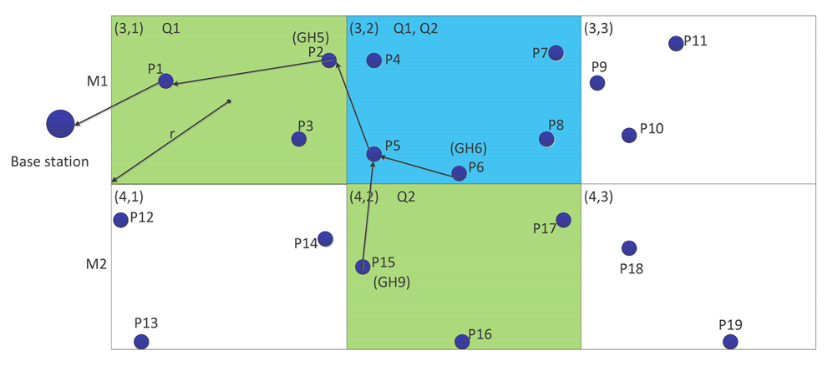
\includegraphics[width=0.7\linewidth]{figs/egf-agg}
	\caption {بازگرداندن داده به \lr{Base Station}}
	\label{fig:egf-agg}
\end{figure}

\par
علاوه بر این، در این مقاله برای تعیین گره‌ی سرگروه هر زیرمحیط از الگوریتم \lr{LEACH} استفاده شده است که با تغییر مداوم سرگروه‌ها از کاهش چشم‌گیر یک گره خاص جلوگیری نموده و منجر به افزایش طول عمر سیستم می‌گردد.

\subsection{درخت ECH}
از بسیاری جهات، رویکرد مقاله \cite{} همانند مقاله‌ی قبلی است. هر دو از رویکرد تجمیع کوئری یکسانی استفاده کرده‌اند، هر دو مدل‌های انرژی و کوئری‌شان یکسان است و هر دو اساس کارشان ساختن درخت برای توپولوژی شبکه مبتنی بر اینترنت اشیا می‌باشد. اما تفاوت عمده این دو رویکرد در نحوه ساخت درختشان است که عملکردشان را متفاوت می‌سازد.

\par
در الگوریتم ارائه شده توسط این مقاله که در شکل \ref{fig:ech-al1} دیده می‌شود، همانند مقاله پیشین، ابتدا محیط به سلول‌های با ضلع $\sqrt{2}r$ تقسیم می‌گردد. سپس سلول‌های تقسیم‌بندی شده، هر یک به عنوان یک زیرمحیط در نظر گرفته می‌شوند و الگوریتم شکل \ref{fig:ech-al2} بر روی آن‌ها اعمال می‌گردد. می‌توان گفت که اساس کار این مقاله، در واقع همین الگوریتم است و تفاوت اصلی رویکرد این مقاله با مقاله‌ی پیشین در همین مرحله رقم می‌خورد. در راهکار ارائه شده در این مقاله، دو عدد ثابت به عنوان حداقل و حداکثر تعداد گره‌های فرزند (و یا در سطوح بالاتر: زیرمحیط‌ها) در یک زیرمحیط در نظر گرفته شده است که به ترتیب، با $m$ و $M$ نمایش داده می‌شوند. الگوریتم شکل \ref{fig:ech-al2} بیان می‌دارد که ابتدا تعداد گره‌های فرزند بررسی می‌شود. اگر تعداد گره‌ها در بازه‌ی $m..M$ بود، همان گره‌ها به عنوان یک زیرمحیط با سطح بالاتر به عنوان خروجی الگوریتم برگردانده می‌شود. اما اگر چنین نبود و تعداد بیش از $M$ باشد؛ تعداد $k$ گره از میان گره‌های فرزند انتخاب می‌شود. لازم به ذکر است که چون تعداد گره‌ها برابر با $num$ و تعداد حداقل و حداکثر فرزندان به ترتیب، برابر با $m$ و $M$ می‌باشد؛ پس مقدار $k$ باید در بازه $num/M..num/m$ قرار داشته باشد.
\par
پس از آن که این انتخاب در بین گره‌های فرزند صورت گرفت. برای هر گره باقی‌مانده وزن آن نسبت به $k$ گره انتخاب شده سنجیده می‌شود و در این بین هر کدام که وزن بیشتری را به عنوان حاصل، به دست آورد؛ آن گره فرزند گره مذکور از بین $k$ گره انتخابی می‌شود و اگر تعداد زیرگره‌ها برای یک گره بیش از $M$ شود. همین الگوریتم روی آن گره مخصوص مجددا اعمال می‌گردد. لازم به ذکر است که الگوریتم محاسبه‌ی وزن دقیقا همانند الگوریتم‌های شکل \ref{fig:egf-al2} و
\ref{fig:egf-al3}
 بوده و این عملیات تا زمانی ادامه می‌یابد که تعداد زیرمحیط‌ها از $m$ بیشتر باشد. به این ترتیب، زمانی که تعداد گره‌ها کمتر از $m$ شد؛ ریشه‌ی درخت مشخص شده و عملیات ساخت درخت پایان می‌یابد.

\par
در پایان می‌توانید درخت ساخته شده توسط الگوریتم ابداعی این مقاله را در شکل \ref{fig:ech-graph} مشاهده نمایید. همان‌گونه که در مقایسه‌ی این درخت با درخت شکل \ref{fig:egf-graph} مشهود است؛ وجه مشابهت هر دو درخت در این است که در هر دوی آن‌ها، سلول‌های تقسیم‌بندی شده‌ی محیط برگ‌های درخت می‌باشند. اما عمده تفاوت این دو درخت این است که درخت به دست آمده از الگوریتم مقاله‌ی \cite{}، درختی متوازن است و عمق کمتری دارد. همین امر می‌تواند سبب کاهش مسیر ارتباطی داده‌ها و درخواست‌ها گردیده و در نتیجه، میزان انرژی مصرفی سیستم‌های مبتنی بر اینترنت اشیا را کاهش دهد.

\begin{figure}
	\centering
	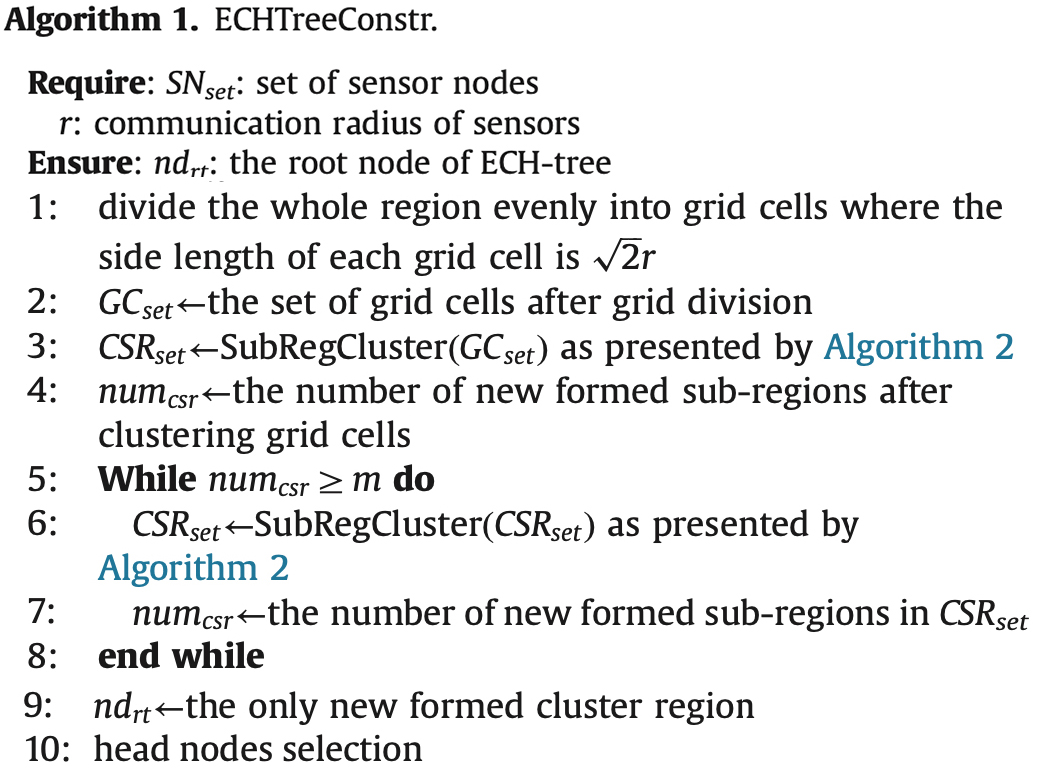
\includegraphics[width=0.7\linewidth]{figs/ech-al1}
	\caption {شبه کد الگوریتم ساخت درخت ECH}
	\label{fig:ech-al1}
\end{figure}

\begin{figure}
	\centering
	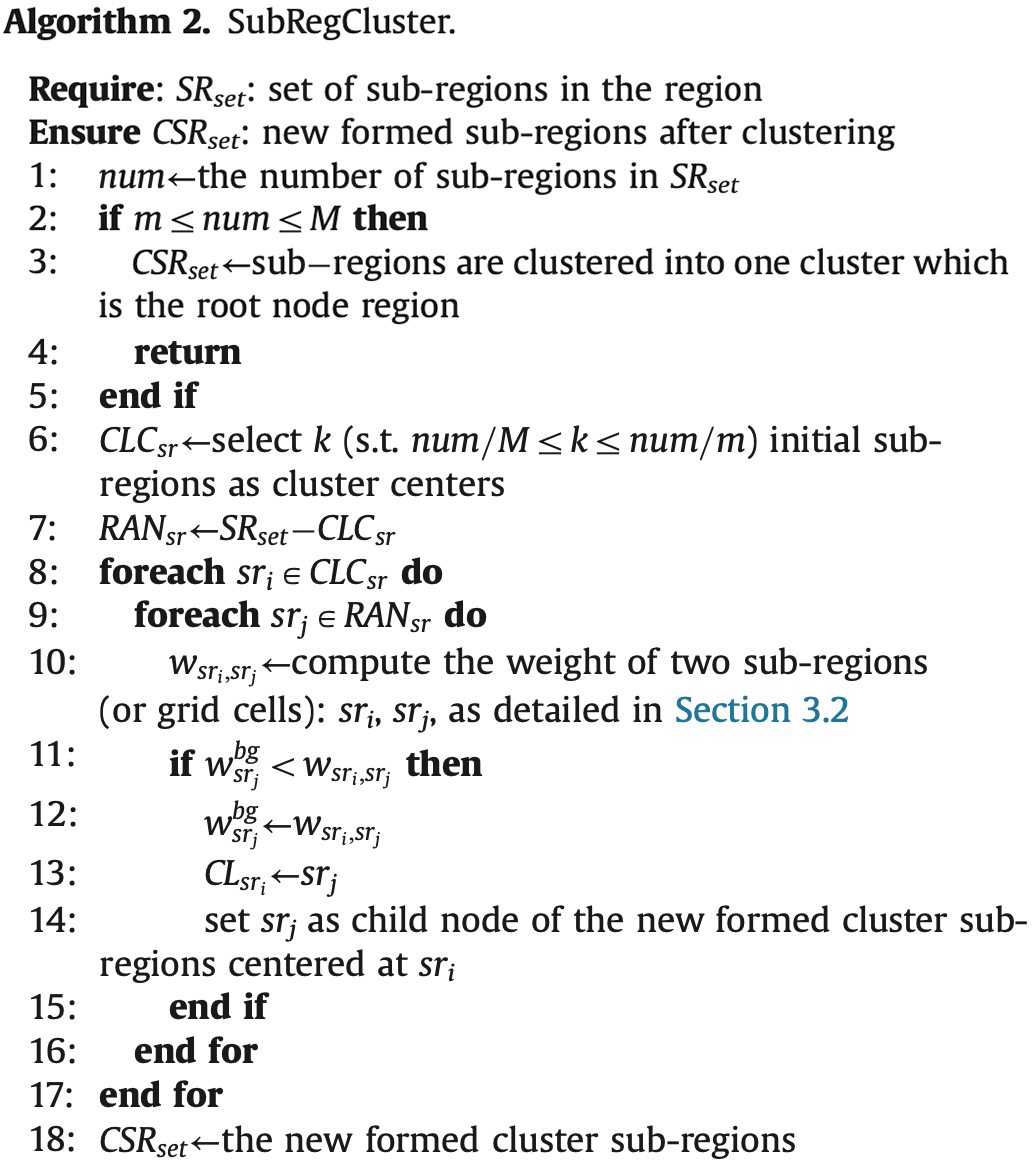
\includegraphics[width=0.7\linewidth]{figs/ech-al2}
	\caption {شبه کد الگوریتم خوشه‌بندی ECH}
	\label{fig:ech-al2}
\end{figure}

\begin{figure}
	\centering
	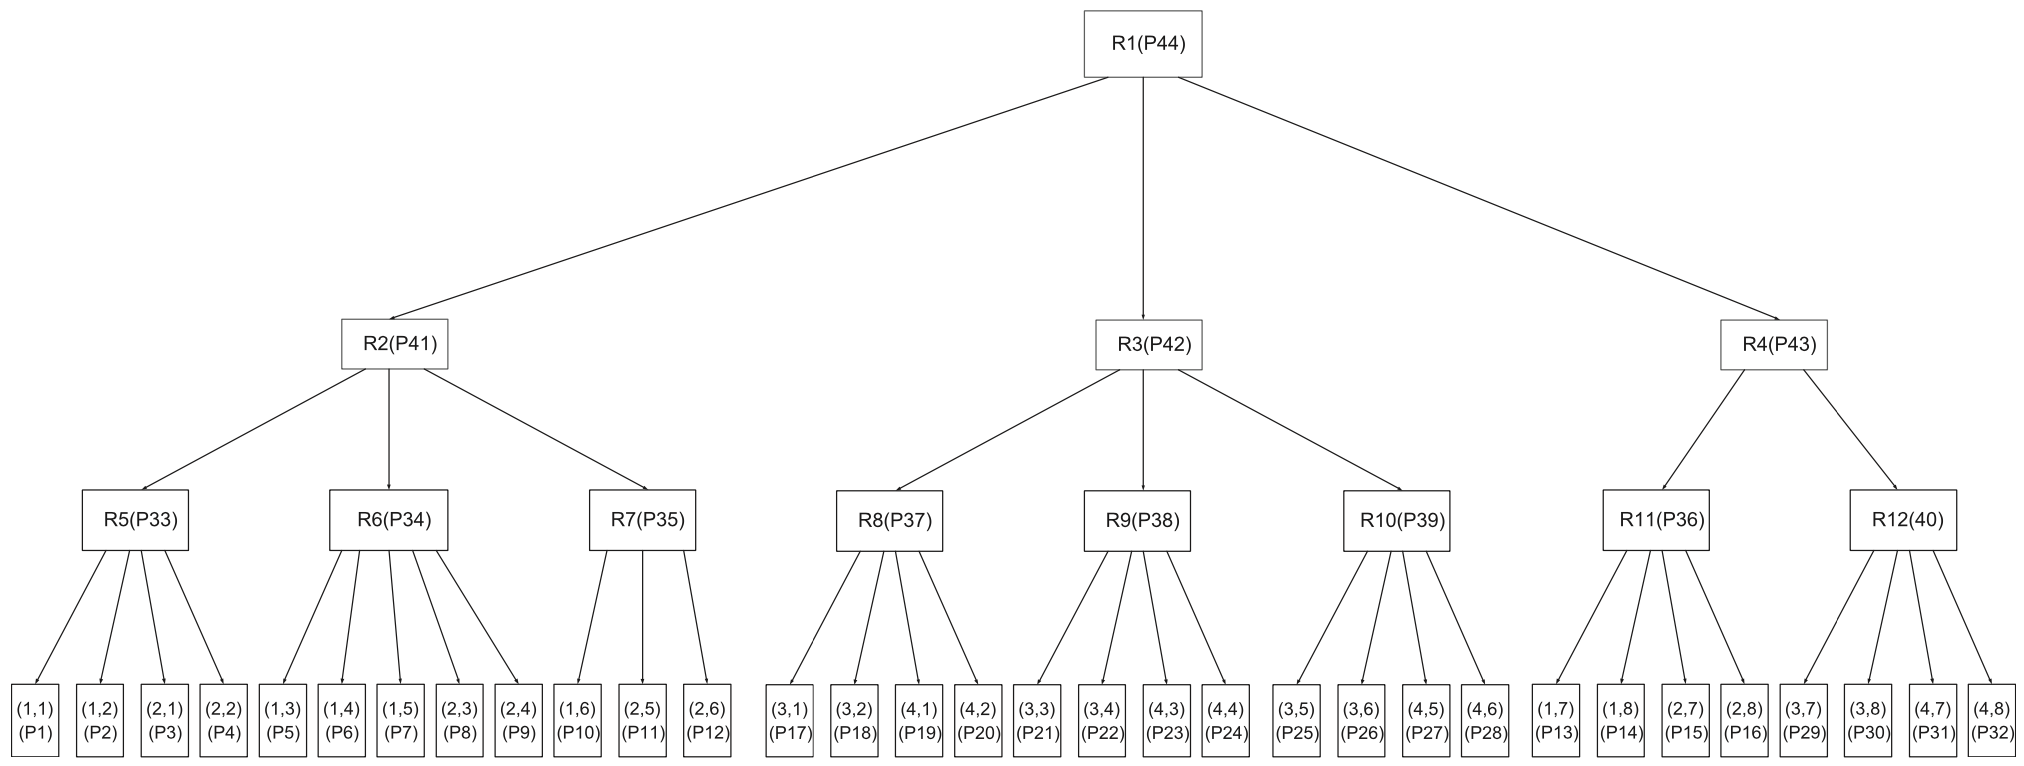
\includegraphics[width=0.7\paperheight,angle=90,origin=c]{figs/ech-graph}
	\caption {گراف ساخته شده با الگوریتم ECH}
	\label{fig:ech-graph}
\end{figure}

\section{راهکار \lr{Object Group Mobility} \lr{(OGM)}}
در راهکار ارائه شده در مقاله‌ی \cite{}، که با نام \lr{Object Group Mobility} معرفی شده است؛ شبکه‌ای از گره‌ها در نظر گرفته شده که می‌توانند در حرکت باشند (موقعیت‌شان را تغییر دهند) و همچنین در محیط مورد بررسی می‌تواند گروه‌های گوناگونی از گره‌ها وجود داشته باشد که فناوری ارتباطی آن‌ها با یکدیگر یکسان نیست. برای مثال در یک گروه ممکن است فناوری ارتباطی \lr{IEEE 802.15.4} به کار رود. در صورتی که در گروهی دیگر از \lr{RFID} و یا \lr{Bluetooth} استفاده می‌شود. پس به همین دلیل می‌توان گفت شبکه‌ی مورد بررسی و به تبع آن، راهکار ارائه شده دارای انعطاف بیشتری است.
\par
در این مقاله، فرض شده که محیط مورد بررسی $A$ متشکل از مجموعه ای از محیط‌های کوچک‌تر است که به آن‌ها \lr{Ambience} گفته می‌شود. ما برای سادگی و یکپارچگی اصطلاحات به‌کار رفته تا بدین جا، از همان لفظ زیرمحیط برای بیان این مفهوم استفاده می‌نماییم. پس محیط $A$ به شکل $A = \{a_1, a_2, \ldots, a_M\}$ قابل بیان است که $a_i$ بیان‌گر زیرمحیط $i$ام می‌باشد.
\par
سیستم ابداعی این مقاله، در واقع متشکل گروه‌هایی است که خود، مجموعه‌ای از \lr{Access Point (AP)}‌های ناهمگن هستند و می‌توانند در کنار یکدیگر کار کنند.  برای مثال اگر سیستم مورد بحث ما یک ساختمان هوشمند باشد، هر یک از واحد‌های آن یک گروه در سیستم ماست. هر یک از \lr{AP}های یک گروه، دارای فناوری ارتباطی مخصوص خودش است که با $\psi(AP)$ نمایش داده می‌شود. علاوه بر این، هر \lr{AP} تعدادی از زیرمحیط‌ها را پوشش می‌دهد که مجموعه‌ی زیرمحیط‌های تحت پوشش آن را با $C(AP)$ نمایش می‌دهند. بدیهی است  که هر حسگر فقط می‌تواند به \lr{AP}هایی وصل شود که فناوری ارتباطی یکسانی با آن داشته باشند.
\par
در راهکار ارائه شده، یک \lr{Content Server (CS)} به کنترل موقعیت حسگر‌ها می‌پردازد و علاوه بر این، هر حسگر دارای یک \lr{Home Network} 
($HN(n)$)
 است که در آن یک \lr{Agent} (که در مقاله با نام \lr{Home Agent} معرفی شده است) مسئول نگه‌داری اطلاعات مربوط به موقعیت حسگر است. برای این‌که به سازوکار ابداعی این مقاله آشنا شویم؛ فرض کنید یک گروه از گره‌ها را در اختیار داریم که آن‌ها را با $n_0, \ldots, n_m$ نمایش می‌دهیم. فرض می‌نماییم که در این گروه، گره $n_0$ به عنوان گره سرگروه انتخاب شده است. هر گره پیرو\LTRfootnote{Slave}، آدرسی که سرگروه به آن نسبت می‌دهد به عنوان \lr{Care-of-Address} خود ($CoA(n_i)$) معرفی می‌نماید. این آدرس در واقع همان $HN(n_0)$ است. بدین ترتیب زمانی که یک گره بخواهد با یکی از گره‌های $n_1, \ldots, n_m$ ارتباط برقرار کند، درخواست خود را (که می‌تواند شامل داده‌های مورد انتقالی و یا ... باشد) به $CoA(n_i)$ ارسال می‌نماید. سپس براساس $CoA(n_i)$ گره مقصد، درخواست به $HN(n_0)$ منتقل\LTRfootnote{Forward} می‌گردد و از آن‌جا توسط $n_0$ برای گره موردنظر ارسال می‌شود.

\par
از راهکار ارائه شده در بالا چنین بر می‌آید که اگر یک گره بخواهد موقعیت خود را تغییر دهد نیازمند به‌روزرسانی تمامی گره‌های پیروی دیگر نبوده و فقط کافیست اطلاعات موجود در $HN$ گره سرگروه به روزرسانی شود. بدیهی است که همین امر سبب کاهش داده‌های انتقالی و در نتیجه کاهش مصرف انرژی در سیستم‌های مبتنی بر اینترنت اشیا می‌گردد.

\par
پس از آنکه جابجایی یک گره در شبکه به وقوع پیوست، گره مذکور اطلاعات خود را از قبیل \lr{IPv6}، 
\lr{MAC Address}،
فناوری ارتباطی ($\psi(n)$)
و در صورتی که گره سرگروه باشد آدرسی که باید برای گره‌های پیرو \lr{Set} شود را به \lr{Content Server} ارسال می‌نماید. \lr{Content Server} دو وظیفه‌ی اصلی بعد از دریافت این اطلاعات از جانب یک گره دارد.

\begin{itemize}
\item{
به‌روزرسانی اطلاعات موقعیت و گروه‌ها: در این مرحله، \lr{CS} بعد از بررسی سازگاری گره اضافه شده به گروه، به‌روزرسانی اطلاعات را انجام می‌دهد. علاوه بر این در همین حین، \lr{CS} بررسی می‌کند که آیا امکان ادغام گروه موردنظر با سایر گروه‌ها وجود دارد یا خیر. به طور کلی، گروهی که گره $n$ در آن قرار دارد 
($\Gamma(n)$)
 اگر یکی از دو شرط مطرح شده را داشته باشد می‌تواند با گروه $\Gamma_i$ ادغام گردد. شرایط بدین شرح است که یا تمام گره‌هایی با فناوری ارتباطی مشابه، اخیرا گروه $\Gamma_i$ را ترک و به گروه $\Gamma(n)$ پیوسته باشند. و یا این که در گروه $\Gamma_i$ دیگر گره‌ای با فناوری ارتباطی مشابه وجود نداشته باشد.
}
\item{
تخمین موقعیت جغرافیایی حسگرها: بر اساس اطلاعات موقعیتی که به \lr{CS} ارسال شده است، \lr{CS} می‌تواند تخمینی در ارتباط با موقعیت جغرافیایی این حسگر داشته باشد. برای مثال اگر گره $n$ به گروه جدیدی بپیوندد؛ به ازای هر گره موجود در گروه جدید ($z$) می‌توان رابطه $\Phi(z) = C(AP(z)$ را معرفی کرد که بیانگر زیرمحیط‌هایی است که گره $z$ آن‌ها را پوشش می‌دهد. در نتیجه بدیهی است که این حسگرها در محیط اشتراکی به دست آمده، یعنی $\bigcap_{z \in \Gamma(n)} \Phi(z)$ قرار دارند. 
}
\end{itemize}

\par
در شکل \ref{fig:ogm-proc} می‌توانید نمودار فرآیند جابجایی حسگرها در راهکار ارائه شده توسط این مقاله را مشاهده نمایید.

\begin{figure}
	\centering
	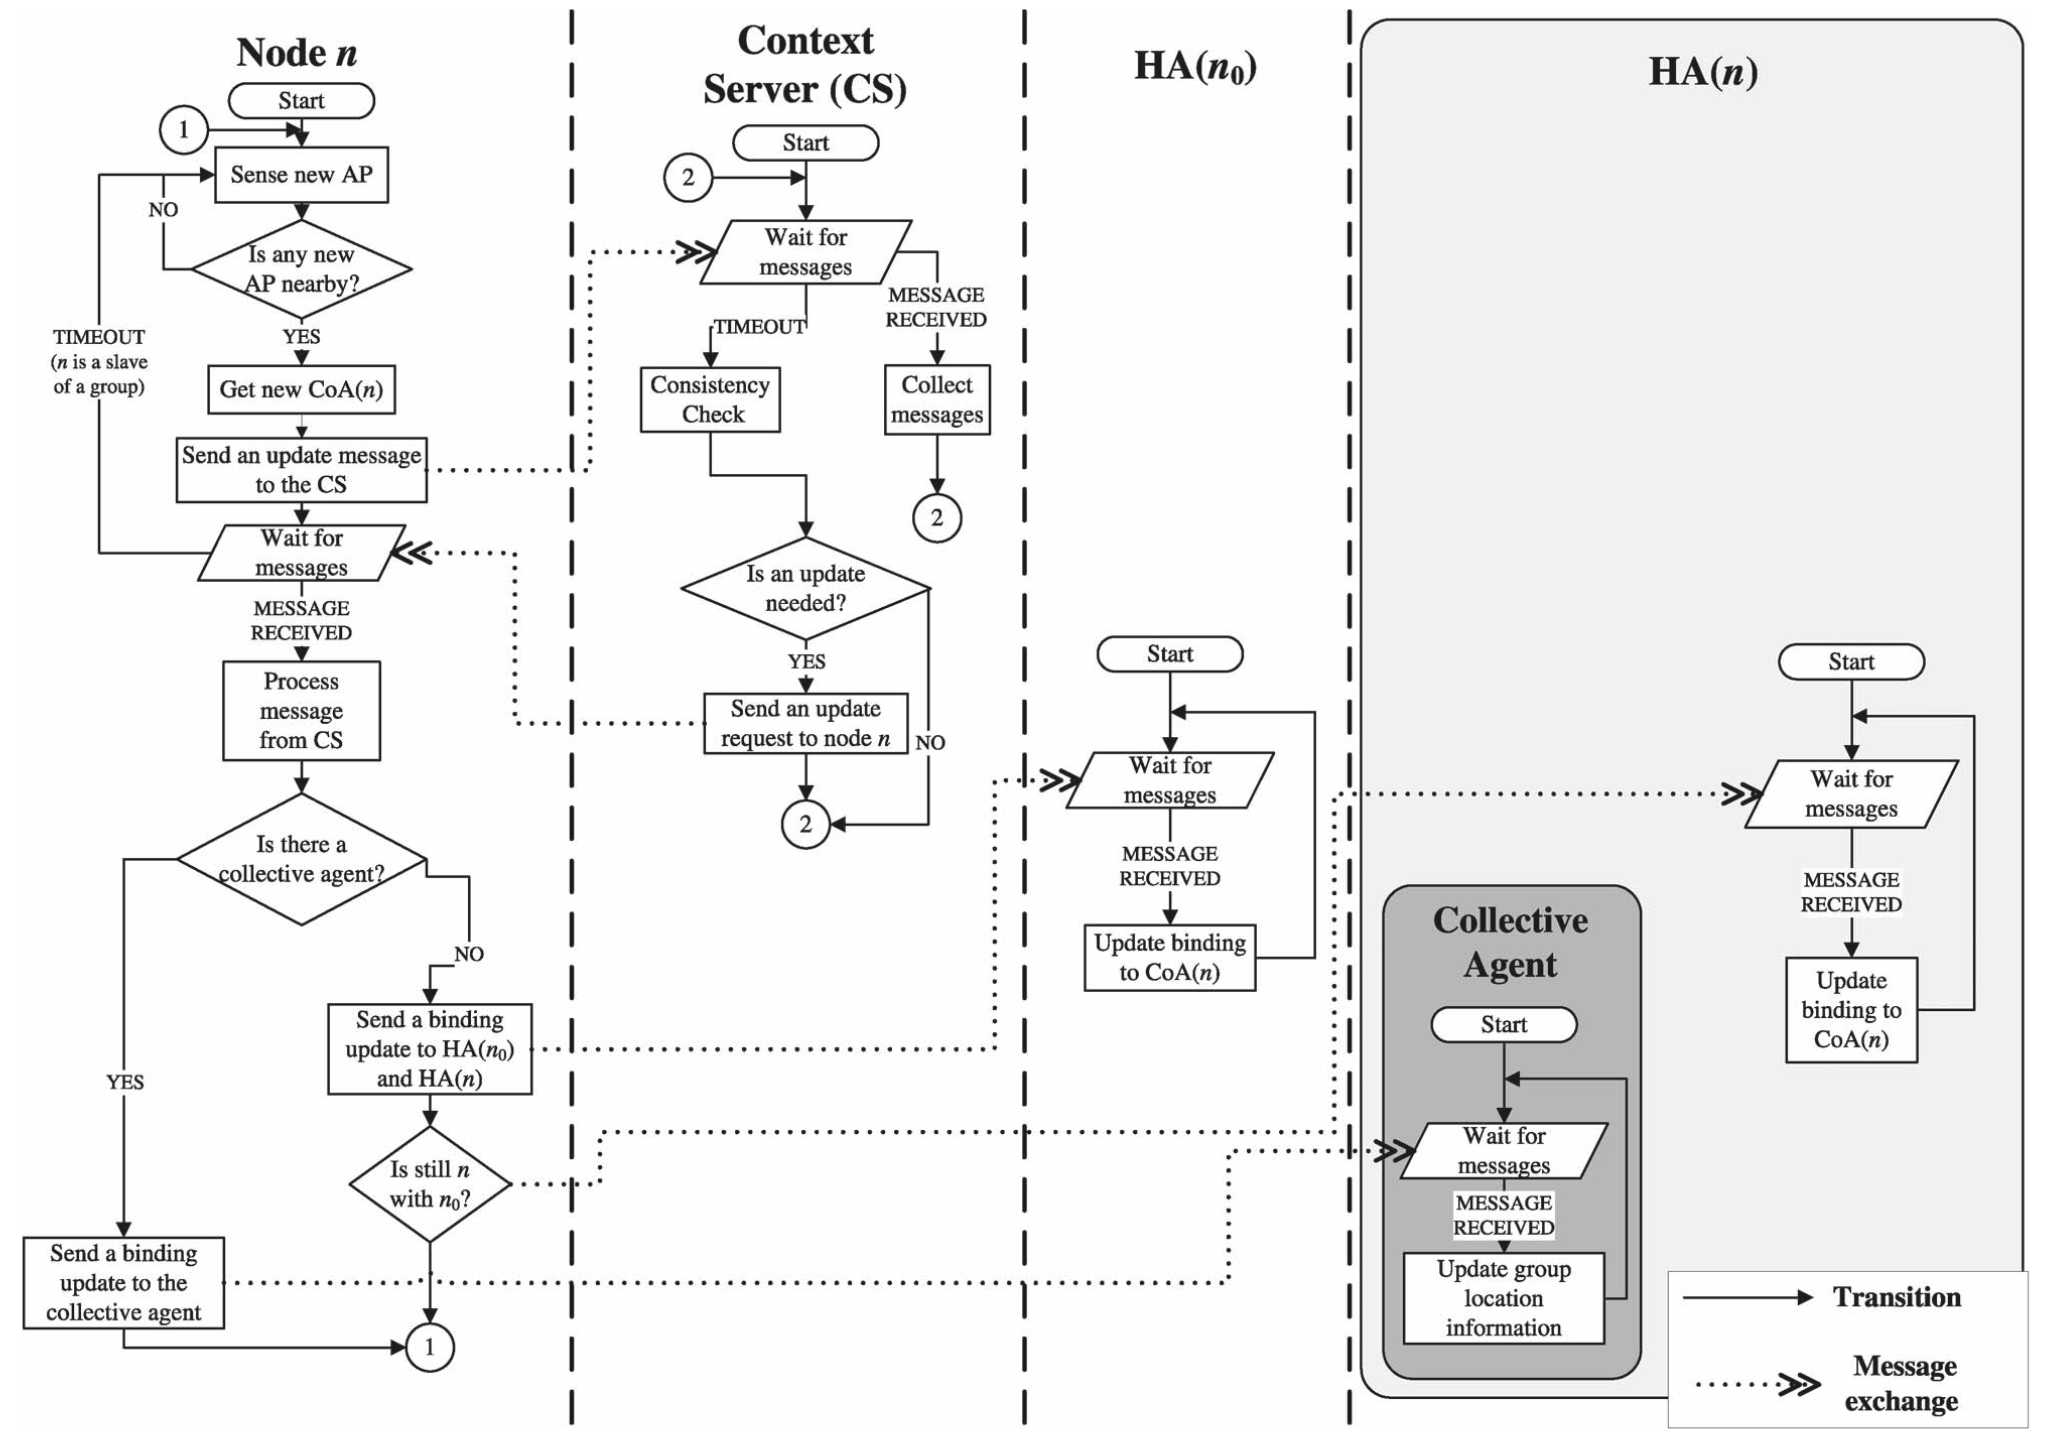
\includegraphics[width=0.9\linewidth]{figs/ogm-proc}
	\caption {فرآیند جابجایی حسگرها در OGM}
	\label{fig:ogm-proc}
\end{figure}

\section{راهکار \lr{Self Organized Things} \lr{(SoT)}}
در راهکار ارائه شده‌ی مقاله‌ی \cite{}، علاوه بر دو هدف اصلی که تا به حال درباره‌ی آن صحبت نموده‌ایم - یعنی کاهش انرژی مصرفی سیستم و به دنبال آن، افزایش طول عمر سیستم - هدف دیگری نیز مدنظر قرار گرفته است و آن کاهش نیازمندی به انسان جهت مدیریت سیستم‌های مبتنی بر اینترنت اشیا می‌باشد.
راهکار ارائه شده در این مقاله، بر اساس سه تابع \lr{Self-Configuration}، 
\lr{Self-Optimization} و \lr{Self-Healing}
رفتار می‌کند که در ادامه به بررسی هریک از آن‌ها می‌پردازیم.

\subsection{تابع \lr{Self-Configuration}}
اولین تابع به کار رفته در سازوکار ارائه شده، تابع \lr{Self-Configuration} است. این تابع همان‌گونه که در شکل \ref{fig:sot-al1} قابل مشاهده است، وظیفه‌ی پیکربندی اولیه سیستم را بر عهده دارد. عملکرد تابع مذکور به این شکل است که هر یک از حسگر‌های \lr{Trigger-Based} را در حالت فعال و تمامی حسگرهای \lr{Periodic} را در حالت خواب قرار می‌دهد. لازم به ذکر است که در این سیستم، حالت هر حسگر (که با $\phi$ نمایش داده می‌شود) بر سه نوع است. خواب\LTRfootnote{Sleep}، بیدار\LTRfootnote{Active} و منفعل (خاموش)\LTRfootnote{Passive}. در حالت خواب، حسگر روشن است اما به پایش و دریافت اطلاعات محیط مشغول نیست و در نتیجه کمترین میزان مصرف انرژی را دارد. در حالت بیدار (فعال)، حسگر روشن است و به پایش محیط می‌پردازد. در حالت خاموش نیز حسگر به طور کلی خاموش است و انرژی‌ای مصرف نمی‌کند.

\begin{figure}
	\centering
	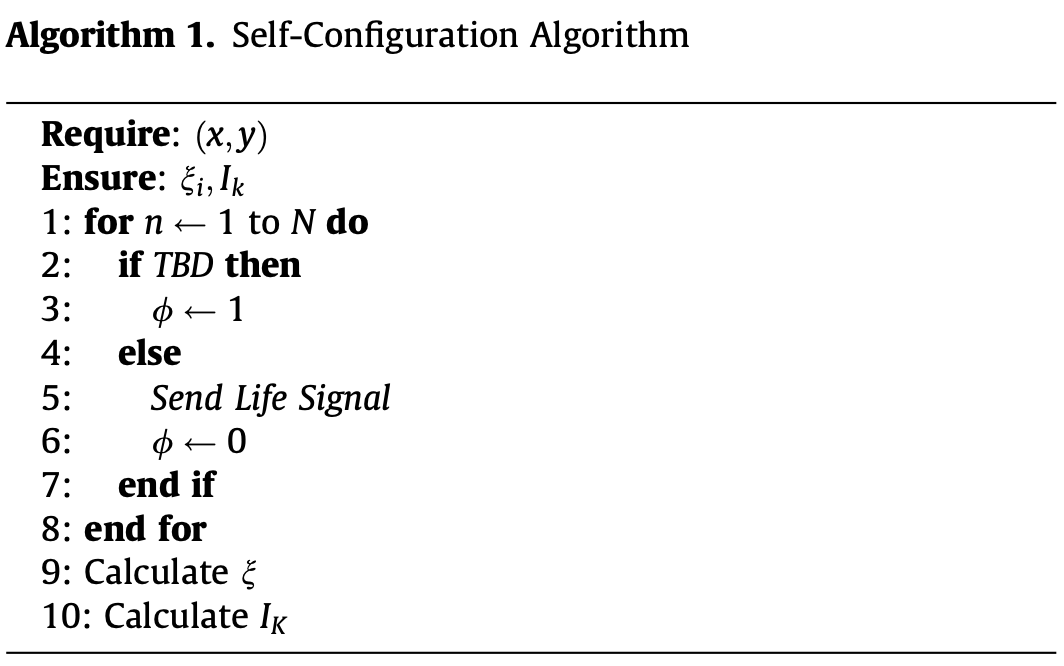
\includegraphics[width=0.7\linewidth]{figs/sot-al1}
	\caption {شبه کد تابع Self-Configuration}
	\label{fig:sot-al1}
\end{figure}

\par
پس از آن که وضعیت هر حسگر بنابر نوع آن تنظیم شد؛ همان‌طور که در خط ۹ و ۱۰ شبه کد شکل \ref{fig:sot-al1} مشاهده می‌شود؛ نوبت به محاسبه‌ی دو پارامتر تعریف شده در این مقاله به ازای هر یک از حسگر‌ها می‌رسد. در ادامه به تعریف این دو پارامتر می‌پردازیم.

\subsubsection{
محاسبه هم‌پوشانی ($\zeta_i$)
}
یکی از پارامترهای معرفی شده در مقاله‌ی مورد بررسی، پارامتری تحت عنوان هم‌پوشانی است که مشخص‌کننده‌ی این است که یک حسگر چه مساحتی را منحصرا تحت پوشش قرار داده است. نحوه‌ی محاسبه‌ی این پارامتر در فرمول \ref{eq:sot-conflict} مشاهده می‌شود. ($D_{ij}$ بیانگر فاصله‌ی بین دو گره $i$ و $j$ است.)

\begin{equation}
\zeta_i = \sum_j \frac{D_{ij} \times 1(D_{ij} < 2R) + 2R \times 1(D_{ij} \geq 2R)}{2R}
\label{eq:sot-conflict}
\end{equation}

\subsubsection{
محاسبه همبستگی فضایی ($I_k$)
}
پارامتر دیگری که در این مقاله به آن اشاره شده، پارامتر همبستگی فضایی\LTRfootnote{Spatial Correlation} می‌باشد. دلیل معرفی این پارامتر این است که پارامتر قبلی (یعنی هم‌پوشانی $\zeta_i$) به تنهایی به موقعیت مکانی حسگرها وابسته است و توجهی به وضعیت حسگرها ندارد. محاسبه‌ی پارامتر همبستگی فضایی در فرمول \ref{eq:sot-spatial} قید شده است.

\begin{equation}
I_k = \frac{\phi_k \times \sum_i \phi_i \times D_{ki}}{\sum_l \phi_l^2}
\label{eq:sot-spatial}
\end{equation}

\subsection{تابع \lr{Self-Optimization}}
پیش از این که به بررسی این تابع بپردازیم، سوالی که پیش می‌آید این است که چرا با وجود پارامتر همبستگی فضایی، نیازمند محاسبه‌ی پارامتر هم‌پوشانی هستیم. در واقع دلیل این امر این است که این پارامتر نسبت به هم‌پوشانی بی‌توجه است و فرض کنید؛ اگر دو حسگر با فاصله از تمامی حسگر‌های دیگر، کنار هم وجود داشته باشند همبستگی فضایی هردوشان بالا می‌رود. حال آن که ممکن است هم‌پوشانی زیادی با یکدیگر داشته باشند.

\par
حال به بررسی عملکرد تابع \lr{Self-Optimization} می‌پردازیم. در تابع مذکور، همان‌طور که در شکل \ref{fig:sot-al2} می‌بینید؛ به ترتیب برای هر یک از حسگرها، مقدار پارامتر هم‌پوشانی‌اش را با تعداد حسگرها فعال شده‌ی محیط مقایسه می‌کنیم. اگر پارامتر هم‌پوشانی با تعداد حسگرها برابر باشد، به این معنی است که حسگر مورد بررسی با حسگرهای پیشین هم‌پوشانی نداشته و در نتیجه فعال می‌گردد. اما اگر پارامتر هم‌پوشانی حسگر تحت بررسی، از تعداد حسگرهای فعال‌شده‌ی محیط کمتر شود؛ به این معنی است که حسگر، با حسگرهای پیشین هم‌پوشانی دارد. در این صورت برای دو حسگری که دارای هم‌پوشانی هستند، دو حالت وجود دارد. اگر پارامتر هم‌پوشانی ($\zeta$) دو حسگر برابر نباشد؛ آن‌گاه حسگری که پارامتر همپوشانی بزرگ‌تری دارد فعال، و حسگر دیگر غیرفعال (خواب) می‌شود. اما اگر دو حسگر، پارامتر هم‌پوشانی برابری داشته باشند؛ در این صورت پارامتر همبستگی فضایی‌شان تعیین‌کننده خواهد بود و حسگری که پارامتر فضایی بیشتری داشته باشد فعال خواهد شد.

\begin{figure}
	\centering
	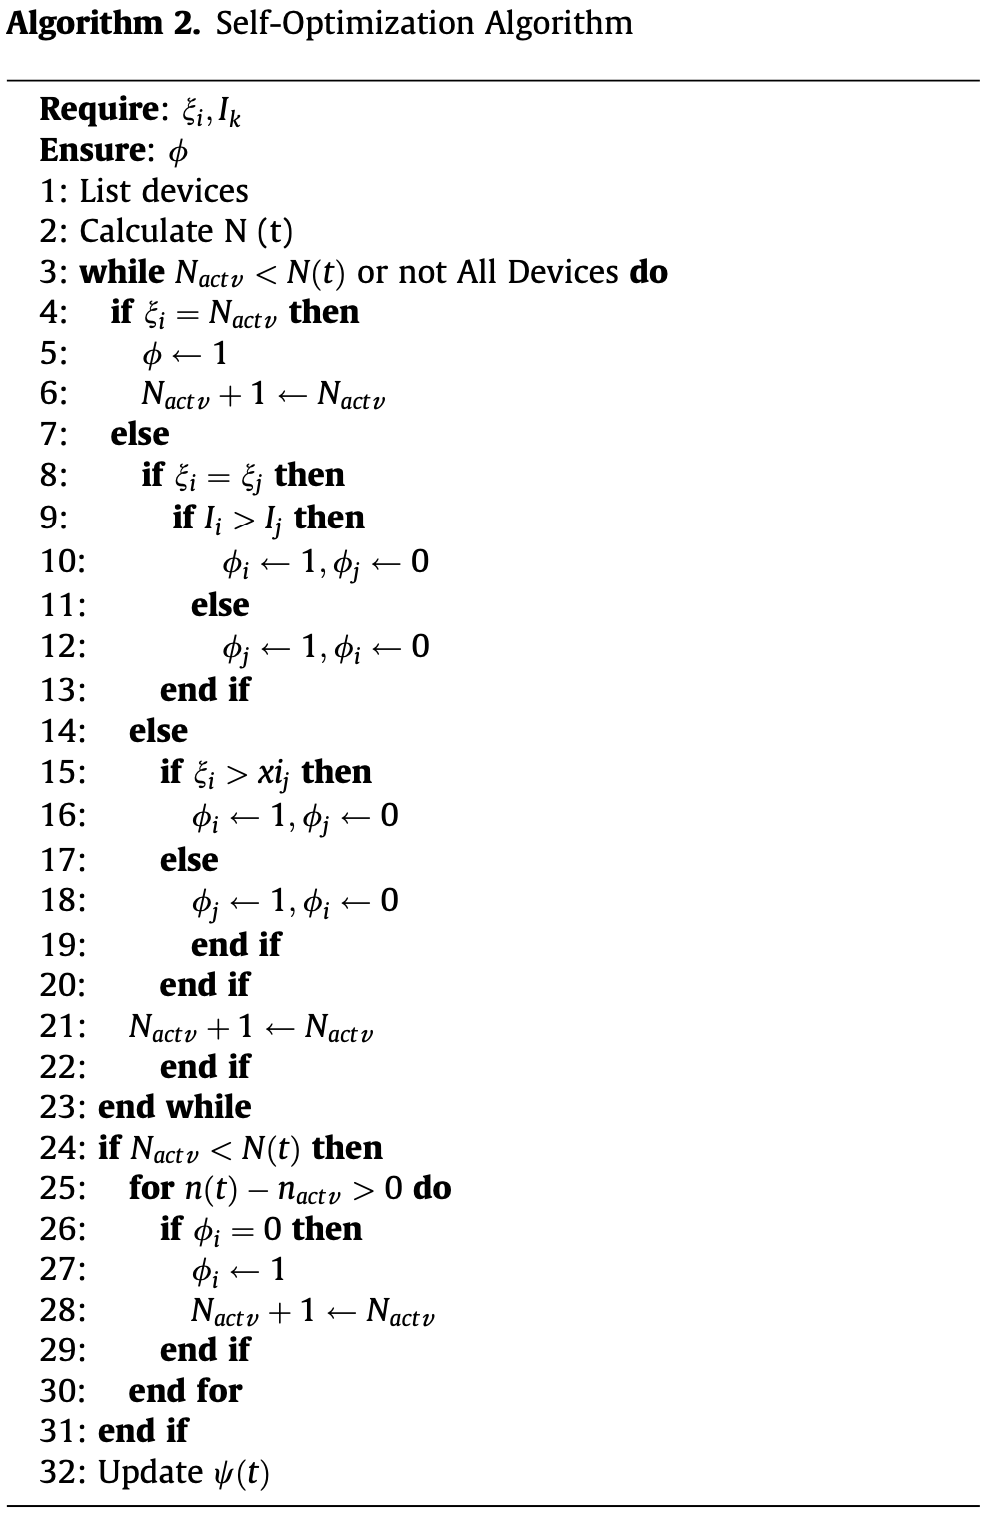
\includegraphics[width=0.7\linewidth]{figs/sot-al2}
	\caption {شبه کد تابع Self-Optimization}
	\label{fig:sot-al2}
\end{figure}

\par
یکی از نکاتی که در ارتباط با تابع فوق مطرح است، این است که همواره از مقدار قبلی پارامتر‌های $\zeta_i$ و $I_k$ برای تعیین وضعیت حسگرها استفاده می‌کند. حال آن که هر یک از تغییرات، خود بر این پارامترها اثر می‌گذارد. نکته‌ای که هست، این است که محاسبه مداوم این پارامترها برای سیستم در حین اعمال تغییرات باعث پیچیدگی محاسباتی سیستم می‌شود. از این رو، برای تعیین وضعیت هر حسگر از آخرین مقدار پارامترهای آن استفاده می‌شود. بدیهی است که این امر موجب کاهش دقت سیستم خواهد گردید. اما آن گونه در مقاله آمده، خطای حاصل از این رویکرد زیاد نبود و قابل چشم‌پوشی است.

\subsection{تابع \lr{Self-Healing}}
تابع خودالتیامی یا همان \lr{Self-Healing}، وظیفه‌اش پایش عملکرد صحیح سیستم است. عملکرد این تابع بسیار شبیه تابع شکل \ref{fig:sot-al1} است. به این صورت که این تابع هر بار که یک سیگنال منفعل (\lr{Passive}) فرستاده می‌شود؛ متوجه می‌گردد که سیستم بهینه نیست. در نتیجه پیکربندی سیستم را از ابتدا انجام داده و پس از حذف حسگر $i$ که مبدا سیگنال \lr{Passive} بوده است، پارامترهای ذکر شده در بالا را برای هر یک از حسگرها مجددا محاسبه می‌نماید.

\subsection{مکانیزم اولویت در سیستم \lr{SoT}}
یکی دیگر از مکانیزم‌های به کار رفته در راهکار مبتنی بر \lr{SoT}، استفاده از اولویت‌بندی برای مخابره‌ی داده توسط حسگرهاست. یکی از مواردی که می‌تواند در سیستم‌های مبتنی بر اشیا، منجر به از دست رفتن داده‌ها بشود، همزمانی ارسال داده از طرف حسگرهای \lr{Trigger-Based} و \lr{Periodic} می‌باشد. بدین منظور، مکانیزمی که در این مقاله، برای  مقابله با چنین خطری تعبیه شده به این صورت است که، هر حسگر \lr{Periodic}، قبل از این که به ارسال داده‌ها بپردازد، به تمامی حسگرهای \lr{Trigger-Based} که با آن هم‌پوشانی دارند سیگنالی ارسال می‌کند که بیانگر فعال شدن حسگر \lr{Periodic} است. حسگرهای \lr{Trigger-Based} با دریافت این سیگنال، غیرفعال شده و شمارنده‌ای را درون خود فعال می‌کنند. زمانی که این شمارنده به صفر برسد؛ این حسگرها مجددا فعال شده و به فعالیت می‌پردازند. همان‌طور که مشاهده می‌شود، در این مکانیزم سعی شده تا هم از تداخل ارسال داده توسط حسگرها جلوگیری شود و هم این که، این امر با حداقل ارتباط میان حسگرها صورت پذیرد. به این معنی که حسگرهای \lr{Trigger-Based} صرفا برای غیرفعال شدن، نیازمند ارسال سیگنال هستند و برای فعال شدن متکی به زمان‌بندی خودشان می‌باشند.

\section{راهکار معماری سه سطحی}
در معماری سه سطحی ارائه شده در مقاله‌ی \cite{}، همان‌طور که در شکل \ref{fig:3l-arch} نیز مشاهده می‌شود، دارای سه سطح هستیم که این سطح‌ها به ترتیب با نام‌های سطح حسگر و کنترل‌کننده\LTRfootnote{Sensing and Controlo Layer (SCL)}، سطح پردازش اطلاعات\LTRfootnote{Information Proccessing Layer (IPL)} و سطح کاربرد\LTRfootnote{Application Layer (AL)} شناخته می‌شوند. وظیفه‌ی سطح اول، پایش محیط و دریافت اطلاعات از آن می‌باشد. این اطلاعات از لایه‌ی اول به لایه‌ی دوم منتقل گشته و در آن‌جا داده‌های ارزشمند از آن استخراج می‌شود. در لایه‌ی سوم نیز اطلاعات به دست آمده از لایه‌ی پیشین به عنوان یک رابط برنامه‌نویسی کاربردی (\lr{API}) در اختیار سایر سرویس‌ها همچون سرویس \lr{Health Monitoring}،
\lr{Smart City}،
\lr{Smart Transportation}
و غیره گذاشته می‌شود تا از اطلاعات حاصل از سیستم مبتنی بر اینترنت اشیا استفاده نمایند. در ادامه، به بررسی عملکرد هر یک از لایه‌های معماری مطرح‌شده می‌پردازیم.

\begin{figure}
	\centering
	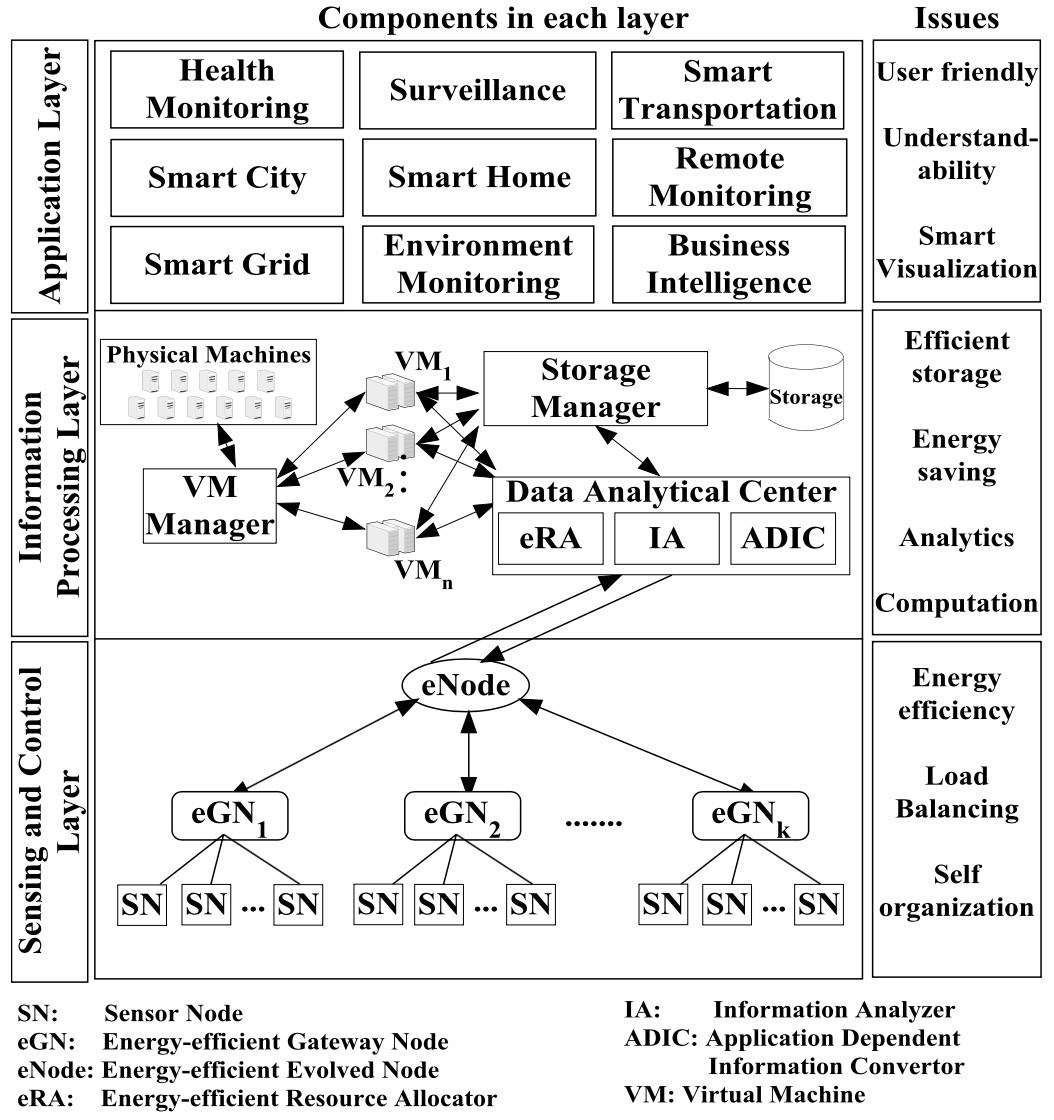
\includegraphics[width=\linewidth]{figs/3l-arch}
	\caption {شمای معماری سه سطحی مقاله \cite{}}
	\label{fig:3l-arch}
\end{figure}

\subsection{لایه‌ی حسگرها و کنترل‌کننده \lr{SCL}}
در این لایه، به طور کلی، سه موجودیت فعالیت دارند. این سه موجودیت به ترتیب حسگرها، \lr{Energy-efficient Gateway Node (eGN)}ها و \lr{Energy-efficient Evolved Node (eNode)} هستند. اگر بخواهیم تصویری کلی از عملکرد این لایه ترسیم کنیم؛ به این شکل است که حسگرها در این سیستم، در زمان‌هایی که کاری برای انجام دادن نداشته باشند؛ غیرفعال می‌شوند. غیرفعال شدن به این معنی است که لایه‌ی ارتباطی آن‌ها غیرفعال شده که در نتیجه، منجر به مصرف انرژی کمتر از جانب آن‌ها می‌گردد. هر حسگر برای فعال شدن مجدد، نیازمند یک سیگنال بیدارباش\LTRfootnote{Wake-Up Signal} از جانب \lr{eGN} خود می‌باشد. \lr{eGN}، تحت سه حالت می‌تواند سیگنال بیدارباش برای یک حسگر ارسال کند. این سه حالت به شرح زیر می‌باشند.

\begin{itemize}
\item{زمانی که مهلت خواب بودن حسگر به پایان برسد.}
\item{زمانی که یک کوئری برای پاسخ‌دهی به آن حسگر ارجاع داده شود.}
\item{زمانی که یک حسگر دیگر، خواستار برقراری ارتباط با آن حسگر باشد.}
\end{itemize}

\par
در مورد اول، حسگر نیازمند استفاده از داده‌هایی است که در زمان خواب بودن از محیط برداشت کرده در حافظه‌ی \lr{Buffer} خود ذخیره کرده است. اما در مورد سوم، حسگر داده‌های دریافت شده از حسگر مبدا را در \lr{Buffer} ذخیره می‌نماید.

\subsubsection{عملکرد \lr{eGN}}
ها،\lr{eGN}
مهمترین بخش در لایه‌ی \lr{SCL} برای کنترل مصرف انرژی هستند. وظیفه‌ی اصلی این گره‌ها، محاسبه‌ی مدت زمان دوره‌های خواب بودن هر حسگر است. برای این کار فرض می‌کنیم که $T^i_{n+1}$، زمان خواب تخمینی حسگر $i$ در دوره‌ی بعد ($n + 1$) و $t^i_{n+1}$، زمان خواب واقعی حسگر $i$ در دوره‌ی بعد باشد. برای محاسبه‌ی این دو پارامتر، به ترتیب از فرمول‌های \ref{eq:3l-T} و \ref{eq:3l-t} استفاده می‌شود.

\begin{equation}
T_{n+1}^i = \alpha t_n^i + (1 - \alpha) T^i_n
\label{eq:3l-T}
\end{equation}

\begin{equation}
t_{n+1}^i = T^i_{n+1} + \Delta t^i
\label{eq:3l-t}
\end{equation}

\par
لازم به ذکر است که در فرمول \ref{eq:3l-T}، پارامتر $\alpha$، بیانگر میزان تاثیر حالت قبلی حسگر نسبت به حالت فعلی بوده و مقدار آن در بازه $0..1$ می‌باشد. این پارامتر بسته به نوع حسگر تعیین می‌شود. برای مثال؛ در حسگرهای \lr{Periodic}، حالت قبلی و فعلی به یک میزان در تعیین $T_{n+1}^i$ اهمیت دارند که در نتیجه باعث می‌شود مقدار $\alpha$ حدودا برابر $0.5$ باشد. اما در حسگرهای \lr{Trigger-Based} که سابقه‌ی سیستم خیلی حائز اهمیت نیست، مقدار 
$\alpha$ 
حدودا برابر صفر تنظیم می‌گردد. علاوه بر این در فرمول \ref{eq:3l-t}، نیازمند محاسبه‌ی پارامتر $\Delta t^i$ هستیم که به برای حسگرهای \lr{Periodic} به شکلی که در فرمول \ref{eq:3l-delta-psd} آمده است؛ محاسبه می‌شود.

\begin{equation}
\Delta t^i = \frac{\oint(k) + \zeta_i}{E_i \times CoV}
\label{eq:3l-delta-psd}
\end{equation}

\par
در فرمول بالا، $\oint(k)$، بیانگر سطح کیفیت داده‌ای حسگر است. در این مقاله نیز همچون روش \lr{MTD} که پیشتر به آن پرداختیم؛ برای کیفیت عملکرد یک حسگر، سطوحی مطرح می‌شود. برای مثال اگر مجموعا ۱۰ سطح کیفیت تعریف گردد و حسگر در سطح پنجم کیفیت باشد (در اینجا، برعکس \lr{MTD}، با افزایش عدد، کیفیت بیشتر می‌گردد.) آن‌گاه مقدار $\oint(k)$ برابر با $0.5$ می‌شود. لازم به ذکر است که این مقدار برای هر حسگر از جانب لایه‌ی \lr{IPL} دریافت می‌گردد. $\zeta_i$، بیانگر پارامتر تداخل\LTRfootnote{Conflict Factor} بوده که مقدار آن معادل 
$\sum_k (2R - D_{ik})$ 
می‌باشد. $E_i$ بیانگر میزان باتری حسگر می‌باشد که به صورت درصدی است و در واقع در بازه‌ی $0..1$ است. هم‌چنین، $CoV$ بیانگر میزان تغییرات داده‌ای است که حسگر در دوره‌های مختلف بازگردانده. فرض کنید مقدار بازگشتی از حسگر مورد نظر ما یک مقدار عددی است؛ در این شرایط، اگر تغییرات این عدد در هر بار پایش محیط، تغییرات زیادی نداشته باشد؛ درمی‌یابیم که نیازی به پایش مداوم آن حسگر نیست. پس \lr{eGN} مدت زمان خواب بودن حسگر را افزایش می‌دهد تا مصرف انرژی حسگر را کاهش دهد. در فرمول \ref{eq:3l-cov} می‌توانید فرمول محاسبه‌ی $CoV$ را مشاهده نمایید. لازم به ذکر است که در این فرمول، $x_i$ برابر مقادیر پایش شده از محیط و $\mu$ بیانگر میانگین داده‌های پایش شده است.

\begin{equation}
CoV = \frac{\sqrt{\sum(x_i - \mu)^2}}{\mu}
\label{eq:3l-cov}
\end{equation}

\par
هم‌چنین، محاسبه‌ی $\Delta t^i$ برای حسگرهای \lr{Trigger-Based} به طریقی که در فرمول \ref{eq:3l-delta-tbd} آمده است؛ صورت می‌گیرد. لازم به ذکر است که
$\Delta\oint$،
بیانگر میزان تغییراتی است که توسط داده‌های ارسالی از حسگر $i$ در سیستم ایجاد می‌شود، $\zeta_i$ همانند فرمول \ref{eq:3l-delta-psd}، بیانگر ضریب تداخل است اما محاسبه‌ی آن کمی متفاوت است و مقدار آن برابر با $\sum_k ((2R - D_{ik}) \times p_i)$ می‌باشد که $p_i$ بیانگر احتمال \lr{Trigger} نشدن حسگر می‌باشد. $E_i$ نیز همانند فرمول پیشین، بیانگر میزان باتری باقی‌مانده حسگر است.

\begin{equation}
\Delta t^i = \frac{\Delta\oint + \zeta_i}{E_i}
\label{eq:3l-delta-tbd}
\end{equation}

\par
پس از آن که محاسبات ذکر شده تا به این جا، توسط \lr{eGN} صورت گرفت، این گره برای هریک از حسگرها که زمان خواب‌شان سپری شده یک سیگنال بیدارباش می‌فرستد. علاوه بر این، در صورتی که حسگری درخواست ارتباط با حسگر تحت کنترل \lr{eGN} را داشته باشد، اگر نیاز باشد تا این ارتباط بلافاصله صورت بگیرد (به عبارت دیگر، ارتباط \lr{Critical} باشد) آن‌گاه \lr{eGN}، سیگنال بیدارباش برای حسگر ارسال می‌کند و ارتباط برقرار می‌گردد. اما در شرایطی که نیازی نباشد تا ارتباط، به صورت بلادرنگ صورت گیرد؛ آن‌گاه داده‌های پیوستی درخواست توسط \lr{eGN} ذخیره شده و پس از فعال شدن حسگر موردنظر در زمان مقرر، این اطلاعات در اختیار آن حسگر قرار می‌گیرد. مجموعه‌ی عملکرد \lr{eGN} که در این بخش تشریح شد را می‌توانید در الگوریتم شکل \ref{fig:3l-al} مشاهده نمایید.

\begin{figure}
	\centering
	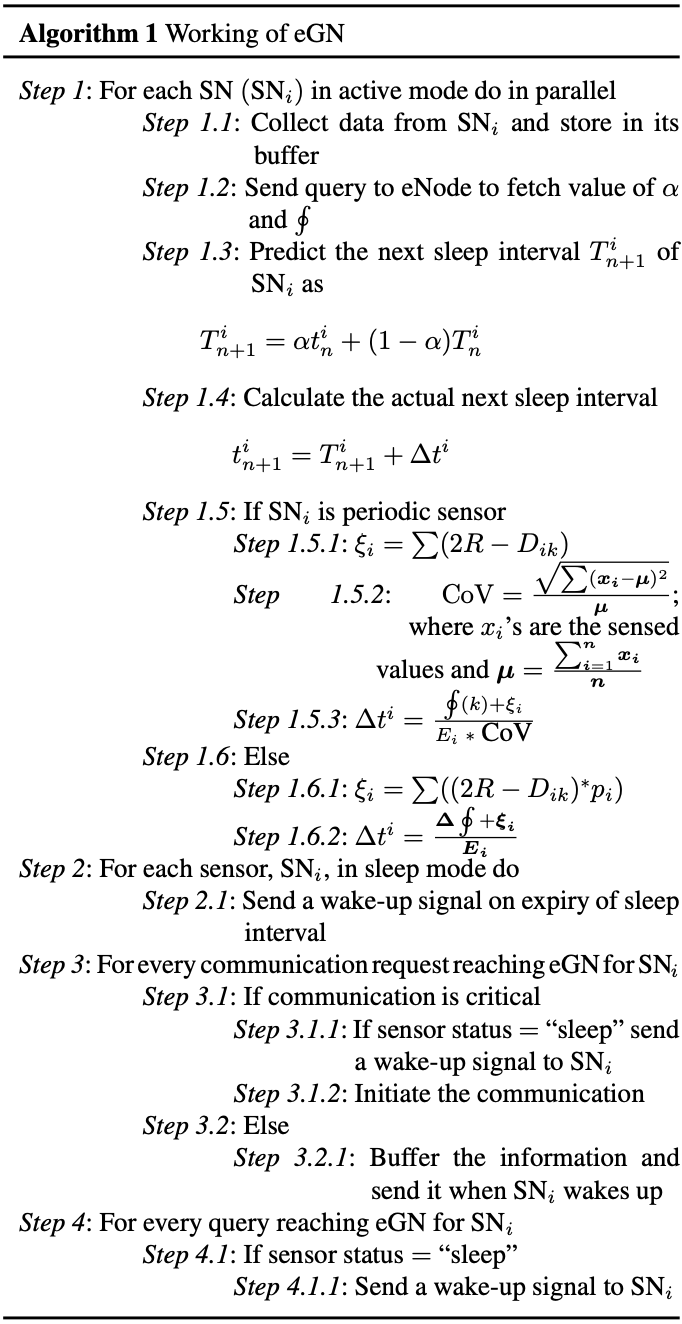
\includegraphics[width=0.7\linewidth]{figs/3l-al}
	\caption {شبه کد الگوریتم عملکرد eGN}
	\label{fig:3l-al}
\end{figure}

\subsubsection{عملکرد eNode}
گره دیگری که در لایه‌ی \lr{SCL} وجود دارد، گره \lr{eNode} است. این گره مسئولیت مدیریت \lr{eGN}های موجود در محیط را داشته و علاوه بر این، وظیفه‌ی انتقال اطلاعات میان لایه‌های \lr{SCL} و \lr{IPL} را بر عهده دارد. برای مثال؛ این گره پارامترهایی همچون $\oint(k)$ که باید از لایه‌ی \lr{IPL} دریافت می‌شد، گرفته و در اختیار \lr{eGN} مربوطه می‌گذارد و در پایان نتایج بازگشتی از حسگرها را به لایه‌ی \lr{IPL} ارسال می‌نماید. در کنار این‌ها، دیگر وظیفه‌ی این گره، تخصیص حسگرها به \lr{eGN}های گوناگون برحسب میزان باتری باقی‌مانده‌ی \lr{eGN} و فاصله‌ی آن‌ها از حسگر می‌باشد. برای محاسبه‌ی پارامتر تخصیص\LTRfootnote{Allocation Factor} از فرمول \ref{eq:3l-aloc} استفاده می‌گردد. لازم به ذکر است که این پارامتر برای هر حسگر، به ازای تمامی \lr{eGN}ها محاسبه گردیده و حسگر به \lr{eGN}ای تخصیص می‌یابد که پارامتر تخصیص آن از همه بیشتر باشد.

\begin{equation}
A(i, k) = \frac{E_k}{D_{ik}}
\label{eq:3l-aloc}
\end{equation}

\subsection{لایه‌ی پردازش اطلاعات \lr{IPL}}
در این لایه مجموعه‌ی گره‌های در حال فعالیت به شرح زیر هستند

\begin{itemize}
\item{
\lr{Energy-efficient Resource Allocator (eRA)}:
این گره، وظیفه صرفه‌جویی در مصرف انرژی توسط منابع \lr{IPL} را برعهده دارد. وظیفه‌ی این گره تخصیص منابع برای داده‌هاست. تخصیص منابع براساس پارامتری به نام $D_{max}$ صورت می‌گیرد که بیانگر حداکثر حجم داده‌ای است که \lr{eNode} برای لایه‌ی \lr{IPL} ارسال می‌نماید.
}
\item{
\lr{Information Analyzer (IA)}:
وظیفه‌ی این بخش محاسبه پارامترهای کیفیت (همانند $\oint(k)$) است که در بخش پیشین به تفصیل آن‌ها را مورد بررسی قرار دادیم.
}
\item{
\lr{Application Dependent Information Convertor (ADIC)}:
این لایه‌، مسئولیت تبدیل داده‌های به دست آمده به قالبی که برای استفاده در لایه‌ی \lr{Application} لازم است؛ بر عهده دارد.
}
\item{
\lr{Physical/Virtual Machines and Storage Media}:
همان‌گونه که از عنوان آن نیز مشخص است؛ این لایه وظیفه‌ی نگه‌داری و ذخیره‌ی داده‌های به دست آمده را بر عهده خواهد داشت.
}
\end{itemize}

\subsection{لایه‌ی کاربرد \lr{AL}}
همان‌طور که پیش‌تر نیز اشاره شده، این لایه مسئولیت ارائه‌ی داده‌های به دست آمده از محیط را به سایر سرویس‌ها همچون
\lr{Health Monitoring}،
\lr{Smart City}،
\lr{Smart Transportation}
و غیره را جهت استفاده از اطلاعات محیط، بر عهده دارد.






















